\documentclass[a4paper]{article}

\usepackage[pdftex,
  hidelinks,
  pdfauthor={Dexter Chua},
  pdfsubject={Cambridge Maths Notes: Part IA - Probability},
  pdftitle={Part IA - Probability},
pdfkeywords={Cambridge Mathematics Maths Math IA Lent Probability}]{hyperref}

\title{Part IA - Probability}
\author{Lectured by R. Weber}
\date{Lent 2015}

% Imports
\ifx \nextra \undefined
  \usepackage[pdftex,
    hidelinks,
    pdfauthor={Dexter Chua},
    pdfsubject={Cambridge Maths Notes: Part \npart\ - \ncourse},
    pdftitle={Part \npart\ - \ncourse},
  pdfkeywords={Cambridge Mathematics Maths Math \npart\ \nterm\ \nyear\ \ncourse}]{hyperref}
  \title{Part \npart\ - \ncourse}
\else
  \usepackage[pdftex,
    hidelinks,
    pdfauthor={Dexter Chua},
    pdfsubject={Cambridge Maths Notes: Part \npart\ - \ncourse\ (\nextra)},
    pdftitle={Part \npart\ - \ncourse\ (\nextra)},
  pdfkeywords={Cambridge Mathematics Maths Math \npart\ \nterm\ \nyear\ \ncourse\ \nextra}]{hyperref}

  \title{Part \npart\ - \ncourse \\ {\Large \nextra}}
\fi

\author{Lectured by \nlecturer \\\small Notes taken by Dexter Chua}
\date{\nterm\ \nyear}

\usepackage{alltt}
\usepackage{amsfonts}
\usepackage{amsmath}
\usepackage{amssymb}
\usepackage{amsthm}
\usepackage{booktabs}
\usepackage{caption}
\usepackage{enumitem}
\usepackage{fancyhdr}
\usepackage{graphicx}
\usepackage{mathtools}
\usepackage{microtype}
\usepackage{multirow}
\usepackage{pdflscape}
\usepackage{pgfplots}
\usepackage{siunitx}
\usepackage{tabularx}
\usepackage{tikz}
\usepackage{tkz-euclide}
\usepackage[normalem]{ulem}
\usepackage[all]{xy}

\pgfplotsset{compat=1.12}

\pagestyle{fancyplain}
\lhead{\emph{\nouppercase{\leftmark}}}
\ifx \nextra \undefined
  \rhead{
    \ifnum\thepage=1
    \else
      \npart\ \ncourse
    \fi}
\else
  \rhead{
    \ifnum\thepage=1
    \else
      \npart\ \ncourse\ (\nextra)
    \fi}
\fi
\usetikzlibrary{arrows}
\usetikzlibrary{decorations.markings}
\usetikzlibrary{decorations.pathmorphing}
\usetikzlibrary{positioning}
\usetikzlibrary{fadings}
\usetikzlibrary{intersections}
\usetikzlibrary{cd}

\newcommand*{\Cdot}{\raisebox{-0.25ex}{\scalebox{1.5}{$\cdot$}}}
\newcommand {\pd}[2][ ]{
  \ifx #1 { }
    \frac{\partial}{\partial #2}
  \else
    \frac{\partial^{#1}}{\partial #2^{#1}}
  \fi
}

% Theorems
\theoremstyle{definition}
\newtheorem*{aim}{Aim}
\newtheorem*{axiom}{Axiom}
\newtheorem*{claim}{Claim}
\newtheorem*{cor}{Corollary}
\newtheorem*{defi}{Definition}
\newtheorem*{eg}{Example}
\newtheorem*{fact}{Fact}
\newtheorem*{law}{Law}
\newtheorem*{lemma}{Lemma}
\newtheorem*{notation}{Notation}
\newtheorem*{prop}{Proposition}
\newtheorem*{thm}{Theorem}

\renewcommand{\labelitemi}{--}
\renewcommand{\labelitemii}{$\circ$}
\renewcommand{\labelenumi}{(\roman{*})}

\let\stdsection\section
\renewcommand\section{\newpage\stdsection}

% Strike through
\def\st{\bgroup \ULdepth=-.55ex \ULset}

% Maths symbols
\newcommand{\bra}{\langle}
\newcommand{\ket}{\rangle}

\newcommand{\N}{\mathbb{N}}
\newcommand{\Z}{\mathbb{Z}}
\newcommand{\Q}{\mathbb{Q}}
\renewcommand{\H}{\mathbb{H}}
\newcommand{\R}{\mathbb{R}}
\newcommand{\C}{\mathbb{C}}
\newcommand{\Prob}{\mathbb{P}}
\renewcommand{\P}{\mathbb{P}}
\newcommand{\E}{\mathbb{E}}
\newcommand{\F}{\mathbb{F}}
\newcommand{\cU}{\mathcal{U}}
\newcommand{\RP}{\mathbb{RP}}
\newcommand{\CP}{\mathbb{CP}}

\newcommand{\ph}{\,\cdot\,}

\DeclareMathOperator{\sech}{sech}
\DeclareMathOperator{\cosech}{cosech}
\DeclareMathOperator{\cosec}{cosec}

\DeclareMathOperator{\covol}{covol}
\DeclareMathOperator{\vol}{vol}

\let\Im\relax
\let\Re\relax
\DeclareMathOperator{\Im}{Im}
\DeclareMathOperator{\Re}{Re}
\DeclareMathOperator{\im}{im}
\DeclareMathOperator{\image}{image}
\DeclareMathOperator{\Ann}{Ann}

\DeclareMathOperator*{\res}{res}
\DeclareMathOperator{\Res}{Res}
\DeclareMathOperator{\Ind}{Ind}

\DeclareMathOperator{\tr}{tr}
\DeclareMathOperator{\diag}{diag}
\DeclareMathOperator{\rank}{rank}
\DeclareMathOperator{\card}{card}
\DeclareMathOperator{\spn}{span}
\DeclareMathOperator{\adj}{adj}

\DeclareMathOperator{\erf}{erf}
\DeclareMathOperator{\erfc}{erfc}

\DeclareMathOperator{\ord}{ord}
\DeclareMathOperator{\Sym}{Sym}

\DeclareMathOperator{\sgn}{sgn}
\DeclareMathOperator{\orb}{orb}
\DeclareMathOperator{\stab}{stab}
\DeclareMathOperator{\ccl}{ccl}

\DeclareMathOperator{\lcm}{lcm}
\DeclareMathOperator{\hcf}{hcf}

\DeclareMathOperator{\Int}{Int}
\DeclareMathOperator{\id}{id}

\DeclareMathOperator{\betaD}{beta}
\DeclareMathOperator{\gammaD}{gamma}
\DeclareMathOperator{\Poisson}{Poisson}
\DeclareMathOperator{\binomial}{binomial}
\DeclareMathOperator{\multinomial}{multinomial}
\DeclareMathOperator{\Bernoulli}{Bernoulli}
\DeclareMathOperator{\like}{like}

\DeclareMathOperator{\var}{var}
\DeclareMathOperator{\cov}{cov}
\DeclareMathOperator{\bias}{bias}
\DeclareMathOperator{\mse}{mse}
\DeclareMathOperator{\corr}{corr}

\DeclareMathOperator{\otp}{otp}
\DeclareMathOperator{\dom}{dom}

\DeclareMathOperator{\Root}{Root}
\DeclareMathOperator{\supp}{supp}
\DeclareMathOperator{\rel}{rel}
\DeclareMathOperator{\Hom}{Hom}
\DeclareMathOperator{\Aut}{Aut}
\DeclareMathOperator{\Gal}{Gal}
\DeclareMathOperator{\Mat}{Mat}
\DeclareMathOperator{\End}{End}
\DeclareMathOperator{\Char}{char}
\DeclareMathOperator{\ev}{ev}
\DeclareMathOperator{\St}{St}
\DeclareMathOperator{\Lk}{Lk}
\DeclareMathOperator{\disc}{disc}
\DeclareMathOperator{\Isom}{Isom}
\DeclareMathOperator{\length}{length}
\DeclareMathOperator{\energy}{energy}
\DeclareMathOperator{\area}{area}
\DeclareMathOperator{\Syl}{Syl}
\DeclareMathOperator{\cl}{cl}
\DeclareMathOperator{\fix}{fix}

\newcommand{\GL}{\mathrm{GL}}
\newcommand{\SL}{\mathrm{SL}}
\newcommand{\PGL}{\mathrm{PGL}}
\newcommand{\PSL}{\mathrm{PSL}}
\newcommand{\PSU}{\mathrm{PSU}}
\newcommand{\Or}{\mathrm{O}}
\newcommand{\SO}{\mathrm{SO}}
\newcommand{\U}{\mathrm{U}}
\newcommand{\SU}{\mathrm{SU}}

\renewcommand{\d}{\mathrm{d}}
\newcommand{\D}{\mathrm{D}}

\tikzset{->/.style = {decoration={markings,
                                  mark=at position 1 with {\arrow[scale=2]{latex'}}},
                      postaction={decorate}}}
\tikzset{<-/.style = {decoration={markings,
                                  mark=at position 0 with {\arrowreversed[scale=2]{latex'}}},
                      postaction={decorate}}}
\tikzset{<->/.style = {decoration={markings,
                                   mark=at position 0 with {\arrowreversed[scale=2]{latex'}},
                                   mark=at position 1 with {\arrow[scale=2]{latex'}}},
                       postaction={decorate}}}
\tikzset{->-/.style = {decoration={markings,
                                   mark=at position #1 with {\arrow[scale=2]{latex'}}},
                       postaction={decorate}}}
\tikzset{-<-/.style = {decoration={markings,
                                   mark=at position #1 with {\arrowreversed[scale=2]{latex'}}},
                       postaction={decorate}}}

\tikzset{circ/.style = {fill, circle, inner sep = 0, minimum size = 3}}
\tikzset{mstate/.style={circle, draw, blue, text=black, minimum width=0.7cm}}

\definecolor{mblue}{rgb}{0.2, 0.3, 0.8}
\definecolor{morange}{rgb}{1, 0.5, 0}
\definecolor{mgreen}{rgb}{0.1, 0.4, 0.2}
\definecolor{mred}{rgb}{0.5, 0, 0}

\def\drawcirculararc(#1,#2)(#3,#4)(#5,#6){%
    \pgfmathsetmacro\cA{(#1*#1+#2*#2-#3*#3-#4*#4)/2}%
    \pgfmathsetmacro\cB{(#1*#1+#2*#2-#5*#5-#6*#6)/2}%
    \pgfmathsetmacro\cy{(\cB*(#1-#3)-\cA*(#1-#5))/%
                        ((#2-#6)*(#1-#3)-(#2-#4)*(#1-#5))}%
    \pgfmathsetmacro\cx{(\cA-\cy*(#2-#4))/(#1-#3)}%
    \pgfmathsetmacro\cr{sqrt((#1-\cx)*(#1-\cx)+(#2-\cy)*(#2-\cy))}%
    \pgfmathsetmacro\cA{atan2(#2-\cy,#1-\cx)}%
    \pgfmathsetmacro\cB{atan2(#6-\cy,#5-\cx)}%
    \pgfmathparse{\cB<\cA}%
    \ifnum\pgfmathresult=1
        \pgfmathsetmacro\cB{\cB+360}%
    \fi
    \draw (#1,#2) arc (\cA:\cB:\cr);%
}
\newcommand\getCoord[3]{\newdimen{#1}\newdimen{#2}\pgfextractx{#1}{\pgfpointanchor{#3}{center}}\pgfextracty{#2}{\pgfpointanchor{#3}{center}}}

\def\Xint#1{\mathchoice
   {\XXint\displaystyle\textstyle{#1}}%
   {\XXint\textstyle\scriptstyle{#1}}%
   {\XXint\scriptstyle\scriptscriptstyle{#1}}%
   {\XXint\scriptscriptstyle\scriptscriptstyle{#1}}%
   \!\int}
\def\XXint#1#2#3{{\setbox0=\hbox{$#1{#2#3}{\int}$}
     \vcenter{\hbox{$#2#3$}}\kern-.5\wd0}}
\def\ddashint{\Xint=}
\def\dashint{\Xint-}


\begin{document}
\maketitle
{\small
  \noindent\textbf{Basic concepts}\\
  Classical probability, equally likely outcomes. Combinatorial analysis, permutations and combinations.  Stirling's formula (asymptotics for $\log n!$ proved).\hspace*{\fill}  [3]
 
  \vspace{10pt}
  \noindent\textbf{Axiomatic approach}\\
  Axioms (countable case). Probability spaces. Inclusion-exclusion formula. Continuity and subadditivity of probability measures. Independence. Binomial, Poisson and geometric distributions. Relation between Poisson and binomial distributions. Conditional probability, Bayes's formula. Examples, including Simpson's paradox.\hspace*{\fill} [5]
 
  \vspace{10pt}
  \noindent\textbf{Discrete random variables}\\
  Expectation. Functions of a random variable, indicator function, variance, standard deviation. Covariance, independence of random variables. Generating functions: sums of independent random variables, random sum formula, moments.
 
  \vspace{5pt}
  \noindent Conditional expectation. Random walks: gambler's ruin, recurrence relations. Difference equations and their solution. Mean time to absorption. Branching processes: generating functions and extinction probability. Combinatorial applications of generating functions.\hspace*{\fill} [7]
 
  \vspace{10pt}
  \noindent\textbf{Continuous random variables}\\
  Distributions and density functions. Expectations; expectation of a function of a random variable.  Uniform, normal and exponential random variables. Memoryless property of exponential distribution.  Joint distributions: transformation of random variables (including Jacobians), examples. Simulation: generating continuous random variables, independent normal random variables. Geometrical probability: Bertrand's paradox, Buffon's needle. Correlation coefficient, bivariate normal random variables.\hspace*{\fill} [6]
 
  \vspace{10pt}
  \noindent\textbf{Inequalities and limits}\\
  Markov's inequality, Chebyshev's inequality. Weak law of large numbers. Convexity: Jensen's inequality for general random variables, AM/GM inequality.
 
  \vspace{5pt}
  \noindent Moment generating functions and statement (no proof) of continuity theorem. Statement of central limit theorem and sketch of proof. Examples, including sampling.\hspace*{\fill} [3]}


\tableofcontents
\setcounter{section}{-1}
\section{Introduction}
In every day life, we often encounter the use of the term probability, and they are used in many different ways. For example, we can hear people say:
\begin{enumerate}
  \item The probability that a fair coin will land heads is $1/2$.
  \item The probability that a selection of 6 members wins the National Lottery Lotto jackpot is 1 in $\binom{19}{6} = 13 983 816$ or $7.15112\times 10^{-8}$.
  \item The probability that a drawing pin will land 'point up' is 0.62.
  \item The probability that a large earthquake will occur on the San Andreas Fault in the next 30 years is about $21\%$
  \item The probability that humanity will be extinct by 2100 is about $50\%$
\end{enumerate}
The first two cases are things derived from logic. We know that the coin either lands heads or tails. By definition, a fair coin is equally likely to land heads or tail. So the probability of either must be $1/2$.

The third is something probably derived from experiments. Perhaps we did 1000 experiments and 620 of the pins point up. The fourth and fifth examples belong to yet another category that talks about are beliefs and predictions.

We call the first kind ``classical probability'', the second kind ``frequentist probability'' and the last ``subjective probability''. In this course, we only consider classical probability.

\section{Classical probability}
\subsection{Classical probability}
\begin{defi}[Classical probability]
  \emph{Classical probability} applies in a situation when there are a finite number of equally likely outcome.
\end{defi}

Consider the problem of points

$A$ and $B$ play a game in which they keep throwing coins. If a head lands, then $A$ gets a point. Otherwise, $B$ gets a point. The first person to get 10 points wins a prize.

Now suppose $A$ has got 8 points and $B$ has got 7. The game has to end because an earthquake struck. How should they divide the prize? We answer this by finding the probability of $A$ winning. Someone must have won by the end of 19 rounds, ie. after 4 more rounds. If $A$ wins at least 2 of them, then $A$ wins.

The number of ways this can happen is $\binom{4}{2} + \binom{4}{3} + \binom{4}{4} = 11$. So $A$ should get $11/16$ of the prize.

\subsection{Sample space and events}
Consider an experiment that has a random outcome.

\begin{defi}[Sample space]
  The set of all possible outcomes is the \emph{sample space}, $\Omega$. We can lists the outcomes as $\omega_1, \omega_2, \cdots \in \Omega$. Each $\omega \in \Omega$ is an \emph{outcome}.
\end{defi}

\begin{defi}[Event]
  A subset of $\Omega$ is called an \emph{event}.
\end{defi}

\begin{defi}[Set notations]
  Given any two events $A, B\subseteq \Omega$,
  \begin{itemize}
    \item The \emph{complement} of $A$ is $A^C = A' = \bar A = \omega\setminus A$.
    \item ``$A$ or $B$'' is the set $A\cup B$.
    \item ``$A$ and $B$''  is the set $A\cap B$.
    \item $A$ and $B$ are \emph{mutually exclusive} or \emph{disjoint} if $A\cap B = \emptyset$.
    \item $A\subseteq B$ means $A\Rightarrow B$.
  \end{itemize}
\end{defi}

\begin{defi}[Probability]
  Suppose $\Omega = \{\omega_1,\omega_2, \cdots, \omega_N\}$. Let $A\subseteq \Omega$ be an event. Then the \emph{probability} of $A$ is
  \[
    \P(A) = \frac{\text{Number of outcomes in } A}{\text{Number of outcomes in }\omega} = \frac{|A|}{N}
  \]
\end{defi}

\begin{eg}
  Suppose $r$ digits are drawn at random from a table of random digits from 0 to 9. What is the probability of
  \begin{enumerate}
    \item No digit exceeds $k$
    \item The largest digit drawn is $k$
  \end{enumerate}

  The sample space is $\Omega = \{(a_1, a_2, \cdots, a_r): 0 \leq a_i \leq 9\}$. Then $|\Omega| = 10^r$.

  Let $A_k = [\text{no digit exceeds }k] = \{(a_1, \cdots, a_r): 0 \leq a_i \leq k\}$. Then $|A_k| = (k + 1)^r$. So $P(A_k) = (k + 1)^r/10^r$.

  Now let $B_k = [\text{largest digit drawn is }k]$. We can find this by finding all outcomes in which no digits exceed $k$, and subtract it by the number of outcomes in which no digit exceeds $k - 1$. So $|B_k| = |A_k| - |A_{k - 1}|$ and $P(B_k) = [(k + 1)^r - k^r]/10^r$.
\end{eg}

\section{Combinatorial analysis}
\subsection{Counting}
\begin{eg}
  A menu has 6 starters, 7 mains and 6 desserts. How many meals are there? Clearly $6 \times 7 \times 6 = 252$.
\end{eg}
This is the fundamental rule of counting:
\begin{thm}[Fundamental rule of counting]
  Suppose we have to make $r$ multiple choices in sequence. There are $m_1$ possibilities for the first choice, $m_2$ possibilities for the second etc. Then the total number of choices is $m_1\times m_2\times \cdots m_r$.
\end{thm}

\begin{eg}
  How many ways can $1, 2, \cdots, n$ be ordered? The first choice has $n$ possibilities, the second has $n - 1$ possibilities etc. So there are $n\times (n - 1)\times\cdots \times 1 = n!$.
\end{eg}

\subsection{Sampling with or without replacement}
Let $N = \{1, 2, \cdots, n\}$ be a list. Let $X = \{1, 2, \cdots, x\}$ be the items. Let $f: N\to X$ with $f(i) =$ item at the $i$th position.

\begin{defi}[1. Sampling with replacement]
  When we sample with replacement, after choosing at item, it is put back and can be chosen again. Then any sampling function $f$ satisfies sampling with replacement.
\end{defi}

\begin{defi}[2. Sampling without replacement]
  After choosing an item, we burn it and cannot choose it again. Then $f$ must be an injective function, and clearly we must have $X \geq n$.
\end{defi}

We can also have sampling with replacement, but we require each item to be chosen at least once. In this case, $f$ must be surjective.

\begin{eg}
  Suppose $N = \{a, b, c\}$ and $X = \{p, q, r, s\}$. How many injective functions are there $N\to X$?

  When we choose $f(a)$, we have 4 options. When we choose $f(b)$, we have 3 left. When we choose $f(c)$, we have 2 choices left. So there are $24$ possible choices.
\end{eg}

\begin{eg}
  I have $n$ keys in my pocket. We select one at random once and try to unlock. What is the possibility that I succeed at the $r$th trial?

  Suppose we do it with replacement. We have to fail the first $r - 1$ trials and succeed in the $r$th. So The probability is
  \[
    \frac{(n - 1)(n - 1) \cdots (n - 1)(1)}{n^r} = \frac{(n - 1)^{r - 1}}{n^r}.
  \]
  Now suppose we are smarter and try without replacement. Then the probability is
  \[
    \frac{(n - 1)(n - 2)\cdots (n - r + 1)(1)}{n(n - 1) \cdots (n - r + 1)} = \frac{1}{n}.
  \]
\end{eg}
\begin{eg}[Birthday problem]
  How many people are needed in a room for there to be a probability of at least a half that two people have the same birthday?

  Suppose $f(r)$ is the probability that, in a room of $r$ people, there is a birthday match.

  We solve this by finding the probability of no match, $1 - f(r)$. The total number of possibilities of birthday combinations is $365^r$. For nobody to have the same birthday, the first person can have any birthday. The second has 364 else to choose, etc.
  \[
    \P(\text{no match}) = \frac{365\cdot 364\cdot 363 \cdots (366 - r)}{365\cdot 365\cdot 365 \cdots 365}
  \]
  If we calculate this with a computer, we find that $f(22) = 0.475695$ and $f(23) = 0.507297$.

  While this might sound odd since 23 is small, we shouldn't be counting the number of people, but the number of pairs. With 23 people, we have $23\times 22/2 = 253$ pairs, which is quite large compared to 365.
\end{eg}
\subsection{Sampling with or without regard to ordering}
Do the labels on the list positions or items matter?

Recall we have the function $f: N\to X$ and they map $f(1), f(2), \cdots, f(n)$.

After choosing the numbers, we can
\begin{itemize}
  \item Leave the list alone
  \item Sort the list ascending. ie. we might get $(2, 5, 4)$ and $(4, 2, 5)$. If we don't care about list positions, these are just equivalent to $(2, 4, 5)$.
  \item Re-number each item by the number of the draw on which it was first seen. For example, we can rename $(2, 5, 2)$ and $(5, 4, 5)$ both as $(1, 2, 1)$. This happens if the labelling of items doesn't matter.
  \item Both of above. So we can rename $(2, 5, 2)$ and $(8, 5, 5)$ both as $(1, 1, 2)$.
\end{itemize}

Combining these four possibilities with whether we have replacement or not, we have 12 possible cases of counting.

\subsection{Four cases of enumerative combinatorics}
\begin{itemize}
  \item Replacement + with ordering: the number of ways is $x^n$.
  \item Without replacement + with ordering: the number of ways is $x_{(n)} = x^{\underline{n}} = x(x - 1)\cdots (x - n + 1)$.
  \item Without replacement + without order: we only care which items get selected. The number of ways is $\binom{x}{n} = C^x_n = x_{(n)}/n!$.
  \item Replacement + without ordering: we only care how many times the item got chosen. We want to find ways to partition $n = n_1 + n_2 + \cdots n_x$. Say $n = 6$ and $x = 3$. We can write a particular partition as
    \[
      **|*|***
    \]
  So we have $n + x - 1$ symbols and $x - 1$ of them are bars. So the number of ways is $\binom{n + x - 1}{x - 1}$.
\end{itemize}
\subsection{Multinomial coefficient}
Suppose we fill successive positions in a list of length $n$, with replacement, from a set of $x$ items. How many ways can this be done so that item $i\in X$ is used $n_i$ times? (of course we must have $n_1 + n_2 + \cdots + n_x = n$.

In the case of $x = 2$, we have the binomial coefficient. In general, we have
\begin{defi}[Multinomial coefficient]
  A \emph{multinomial coefficient} is
  \[
    \binom{n}{n_1, n_2, \cdots, n_x} = \binom{n}{n_1}\binom{n - n_1}{n_2}\cdots \binom{n - n_1\cdots - n_{x - 1}}{n_x} = \frac{n!}{n_1!n_2!\cdots n_x!}.
  \]
  It is the number of ways to distribute $x$ items into $n$ positions with replacement, in which the $i$th position has $n_i$ items.
\end{defi}

\begin{eg}
  We know that
  \[
    (x + y)^n = x^n + \binom{n}{1}x^{n - 1}y + \cdots + y^n.
  \]
  If we have a trinomial, then
  \[
    (x + y + z)^n = \sum_{n_1, n_2, n_3} \binom{n}{n_1, n_2, n_3} x^{n_1}y^{n_2}y^{n_3}.
  \]
\end{eg}

\begin{eg}
  How many ways can we deal 52 cards to 4 player, each with a hand of 13? There are
  \[
    \binom{52}{13, 13, 13, 13} = \frac{52!}{(13!)^4} = 53644737765488792839237440000 = 5.36\times 10^{28}.
  \]
\end{eg}
While computers are still capable of calculating that, what if we have more cards? Suppose each person has $n$ cards. Then the number of ways is
\[
  \frac{(4n)!}{(n!)^4} = \frac{2^{8n}}{\sqrt{2} (\pi n)^{3/2}}.
\]
We can use Stirling's Formula to approximate it:
\subsection{Stirling's formula}
Before we state and prove Stirling's formula, we prove a weaker (but examinable) version:
\begin{prop}
  $\log n!\sim n\log n$
\end{prop}
\begin{proof}
  Note that
  \[
    e^n = 1 + n + \frac{n^2}{2!} + \cdots + \frac{n^n}{n!} + \cdots.
  \]
  So $1 \leq n^n/n! \leq e^n$. Note that
  \[
    \log n! = \sum_{k=1}^n \log k.
  \]
  Now we claim that
  \[
    \int_1^n \log x\;\d x \leq \sum_1^n \log k\leq \int_1^{n + 1}\log x\;\d x.
  \]
  This is true by considering the diagram:
  \begin{center}
    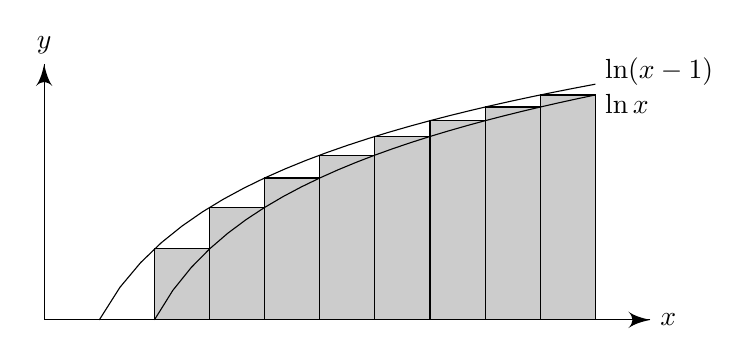
\begin{tikzpicture}[xscale=0.7, yscale=1.3]
     \draw [->] (0, 0) -- (11, 0) node [right] {$x$};
     \draw [->] (0, 0) -- (0, 2.5) node [above] {$y$};
     \draw [domain=2:10] plot (\x, {ln (\x - 1)}) node [anchor = south west] {$\ln (x - 1)$};
     \draw [domain=1:10] plot (\x, {ln \x }) node [anchor = north west] {$\ln x$};
     \draw [fill = black, fill opacity=0.2] (2, 0)-- (2, 0.693147180559945) -- (3, 0.693147180559945) -- (3, 0);
     \draw [fill = black, fill opacity=0.2] (3, 0)-- (3, 1.09861228866811) -- (4, 1.09861228866811) -- (4, 0);
     \draw [fill = black, fill opacity=0.2] (4, 0)-- (4, 1.38629436111989) -- (5, 1.38629436111989) -- (5, 0);
     \draw [fill = black, fill opacity=0.2] (5, 0)-- (5, 1.6094379124341) -- (6, 1.6094379124341) -- (6, 0);
     \draw [fill = black, fill opacity=0.2] (6, 0)-- (6, 1.79175946922806) -- (7, 1.79175946922806) -- (7, 0);
     \draw [fill = black, fill opacity=0.2] (7, 0)-- (7, 1.94591014905531) -- (8, 1.94591014905531) -- (8, 0);
     \draw [fill = black, fill opacity=0.2] (8, 0)-- (8, 2.07944154167984) -- (9, 2.07944154167984) -- (9, 0);
     \draw [fill = black, fill opacity=0.2] (9, 0)-- (9, 2.19722457733622) -- (10, 2.19722457733622) -- (10, 0);
    \end{tikzpicture}
  \end{center}
  Perform the integral to obtain
  \[
    n\log n - n + 1 \leq \log n! \leq (n+ 1)\log (n + 1) - n;
  \]
  Divide both sides by $n\log n$ and let $n\to \infty$. Both sides tend to $1$. So 
  \[
    \frac{\log n!}{n\log n} \to 1.
  \]
\end{proof}

Now we prove Stirling's Formula:
\begin{thm}[Stirling's formula]
  As $n\to \infty$,
  \[
    \log\left(\frac{n! e^n}{n^{n + \frac{1}{2}}}\right) = \log \sqrt{2\pi} + O\left(\frac{1}{n}\right)
  \]
\end{thm}
\begin{cor}
  \[
    n!\sim \sqrt{2\pi}n^{n + \frac{1}{2}} e^{-n}
  \]
\end{cor}
\begin{proof}(non-examinable)
  Define 
  \[
    d_n = \log \left(\frac{n!e^n}{n^{n + 1/2}}\right) = \log n! - (n + 1/2)\log n + n
  \]
  Then
  \[
    d_n - d_{n + 1} = (n + 1/2)\log\left(\frac{n + 1}{n}\right)
  \]
  Write $t = 1/(2n + 1)$. Then
  \[
    d_n - d_{n + 1} = \frac{1}{2t}\log\left(\frac{1 + t}{1 - t}\right).
  \]
  We can simplifying by noting that
  \begin{align*}
    \log (1 + t) - t &= -\frac{1}{2}t^2 + \frac{1}{3}t^3 - \frac{1}{4}t^4 + \cdots\\
    \log (1 - t) + t &= -\frac{1}{2}t^2 - \frac{1}{3}t^3 - \frac{1}{4}t^4 - \cdots
  \end{align*}
  Then if we subtract the equations and divide by $2t$, we obtain
  \begin{align*}
    d_n - d_{n + 1} &= \frac{1}{3}t^2 + \frac{1}{5}t^4 + \frac{1}{7}t^6\\
    &\leq \frac{1}{3}t^2 + \frac{1}{3}t^4 + \frac{1}{3}t^6 = \cdots\\
    &= \frac{1}{3}\frac{t^2}{1 - t^2}\\
    &= \frac{1}{3}\frac{1}{(2n + 1)^2 - 1}\\
    &= \frac{1}{12}\left(\frac{1}{n} - \frac{1}{n + 1}\right)
  \end{align*}
  By summing these bounds, we know that
  \[
    d_1 - d_n \leq \frac{1}{12}\left(1 - \frac{1}{n}\right)
  \]
  Then we know that $d_n$ is bounded below by $d_1 +$ something, and is decreasing since $d_n - d_{n + 1}$ is positive. So it converges to a limit $A$.

  Suppose $m > n$. Then $d_n - d_m < \left(\frac{1}{n} - \frac{1}{m}\right)\frac{1}{12} - \frac{2}{15}\frac{1}{(2n + 1)^4}$ by adding back the term we removed when changing $t^4/5$ to $t^4/3$. So taking the limit as $m\to \infty$, $A < d_n < A + 1/(12n)$, with strict inequalities due to the second term.

  To find $A$, we have a small detour to prove a formula:

  Take $I_n = \int_0^{\pi/2} \sin^n\theta\;\d \theta$. This is decreasing as $n$ increases as $\sin^n\theta$ gets smaller. We also know that
  \begin{align*}
    I_n &= \int_0^{\pi/2}\sin^n \theta\;\d \theta\\
    &= -\cos\theta\sin^{n - 1}\theta |_0^{\pi/2} + \int_0^{\pi/2} (n - 1)\cos^2\theta \sin^{n - 2}\theta \;\d\theta\\
    &= (n - 1)(I_n - 2 - I_n)
  \end{align*}
  So
  \[
    I_n = \frac{n - 1}{n}I_{n - 2}.
  \]
  We can directly evaluate the integral to obtain $I_0 = \pi/2$, $I_1 = 1$. Then
  \begin{align*}
    I_{2n} &= \frac{1}{2}\cdot\frac{3}{4}\cdots \frac{2n - 1}{2n} \pi/2 = \frac{(2n)!}{(2^nn!)^2}\frac{\pi}{2}\\
    I_{2n + 1} &= \frac{2}{3}\cdot\frac{4}{5}\cdots\frac{2n}{2n + 1} = \frac{(2^nn!)^2}{(2n + 1)!}
  \end{align*}
  So using the fact that $I_n$ is decreasing, we know that
  \[
    1 \leq \frac{I_{2n}}{I_{2n + 1}} \leq \frac{I_{2n - 1}}{I_{2n + 1}} = 1 + \frac{1}{2n} \to 1.
  \]
  Using the approximation $n!\sim n^{n + 1/2}e^{-n + A}$, where $A$ is the limit we want to find, we can approximate
  \[
    \frac{I_{2n}}{I_{2n + 1}} = \pi(2n + 1)\left[\frac{( (2n)!)^2}{2^{4n + 1}(n!)^4}\right] \sim \pi(2n + 1)\frac{1}{ne^{2A}}\to \frac{2\pi}{e^{2A}}.
  \]
  Since the last expression is equal to 1, we know that $A = \log\sqrt{2\pi}$
\end{proof}

\begin{eg}
  Suppose we toss a coin $2n$ times. What is the probability of equal number of heads and tails? The probability is
  \[
    \frac{\binom{2n}{n}}{2^{2n}} = \frac{(2n)!}{(n!)^2 2^{2n}} \sim \frac{1}{\sqrt{n\pi}}
  \]
\end{eg}

This approximation can be improved:
\begin{prop}[non-examinable]
  We use the $1/12n$ term from the proof above to get a better approximation:
  \[
    \sqrt{2\pi}n^{n + 1/2}e^{-n} + \frac{1}{12n + 1} \leq n! \leq \sqrt{2\pi} n^{n + 1/2} e^{-n} + \frac{1}{12n}.
  \]
\end{prop}

\begin{eg}
  Suppose we draw 26 cards from 52. What is the probability of getting 13 reds and 13 blacks? The probability is
  \[
    \frac{\binom{26}{13}\binom{26}{13}}{\binom{52}{26}} = 0.2181.
  \]
\end{eg}
\section{Axiomatic approach}
\begin{defi}[Probability space]
  A \emph{probability space} is a triple $(\Omega, \F, P)$. $\Omega$ is the \emph{sample space}, $\F$ is a collection of subsets of $\Omega$. $P: \F\to [0, 1]$ is the \emph{probability measure}. $\F$ has to satisfy the following axioms:
  \begin{enumerate}
    \item $\emptyset, \Omega\in \mathbf{F}$.
    \item $A\in \F \Rightarrow  A^C\in \F$.
    \item $A_1, A_2, \cdots, \in \F \Rightarrow \bigcup_{i = 1}^\infty \in \F$.
  \end{enumerate}
  And $\P$ has to satisfy the following \emph{Kolmogorov axioms}:
  \begin{enumerate}
    \item $0 \leq \P(A) \leq 1 $ for all $A\in \F$
    \item $\P(\Omega) = 1$
    \item For any countable collection of events $A_1, A_2, \cdots$ which are disjoint, ie. $A_i\cap A_j = \emptyset$ for all $i, j$, then
      \[
        \P\left(\bigcup_i A_i\right) = \sum_i \P(A_i).
      \]
  \end{enumerate}
  We say $\P(A)$ is the probability of the event $A$.
\end{defi}

\begin{defi}[Probability distribution]
  Let $\Omega = \{\omega_1, \omega_2, \cdots\}$. Choose $\{p_1, p_2, \cdots, \}$ such that $\sum_{i}^\infty = 1$. Let $p(\omega_i) = p_i$. Then define
  \[
    P(A) = \sum_{\omega_i\in A} p(\omega_i).
  \]
  This $P(A)$ satisfies the above axioms, and $p_1, p_2, \cdots$ is the \emph{probability distribution}
\end{defi}

\begin{thm}\leavevmode
  \begin{enumerate}
    \item $P(\emptyset) = 0$
    \item $P(A^C) + 1 - P(A)$
    \item $A\subseteq B \Rightarrow P(A) \leq P(B)$
    \item $P (A\subseteq B) = P(A) + P(B) - P(A\cap B)$.
    \item Let $A_1\subseteq A_2\subseteq A_3\subseteq \cdots$. Then
      \[
        P\left(\bigcup_1^\infty A_i\right) = \lim_{n\to \infty} P(A_n).
      \]
      This states that $P$ is a continuous set function.
  \end{enumerate}
\end{thm}

\begin{proof}\leavevmode
  \begin{enumerate}
    \item $\Omega$ and $\emptyset$ are disjoint. So $P(\Omega) + P(\emptyset) = P(\Omega \cup \emptyset) = P(\Omega)$. So $P(\emptyset) = 0$.
    \item $P(\Omega) = 1 = P(A) + P(A^C)$ since $A$ and $A^C$ are disjoint.
    \item Write $B = A\cup (B\cap A^C)$. Then $P(B) = P(A) + P(B\cap A^C) \geq P(A)$.
    \item $P(A\cup B) = P(A) + P(B\cap A^C)$. We also know that $P(B) = P(A\cap B) + P(B\cap A^C)$. Then the result follows.
    \item cf. Lecture 7
  \end{enumerate}
\end{proof}

From above, we know that $P(A\cup B) \leq P(A) + P(B)$. So we say that $P$ is a \emph{subadditive} function.  We also know that $P(A\cap B) + P(A \cup B) \leq P(A) + P(B)$ (in fact they are equal!). We say $P$ is \emph{submodular}.

\subsection{Boole's inequality}
This is also known as the ``union bound''.
\begin{thm}[Boole's inequality]
  For any $A_1, A_2, \cdots$,
  \[
    P\left(\bigcup_{i = 1}^\infty A_i\right) \leq \sum_{i =1}^\infty P(A_i).
  \]
\end{thm}

\begin{proof}
  The axiom states a similar formula that only holds for disjoint sets. So we need a clever trick to make them disjoint. We define
  \begin{align*}
    B_1 &= A_1\\
    B_2 &= A_2\setminus B_1\\
    B_i &= A_i\setminus \bigcup_{k = 1}^{i -1 }A_k.
  \end{align*}
  So we know that
  \[
    \bigcup B_i = \bigcup A_i.
  \]
  But the $B_i$ are disjoint. So our Axiom (iii) gives
  \[
    P(\bigcup_i A_i) = P(\bigcup _i B_i) = \sum_i P(B_i) \leq \sum_i P(A_i).
  \]
  Where the last inequality follows from (iii) of the theorem above.
\end{proof}

\begin{eg}
  Suppose we have countably infinite number of biased coins. Let $A_k = [k$th toss head$]$ and $P(A_k) = p_k$. Suppose $\sum_1^\infty p_k < \infty$. What is the probability that there are infinitely many heads?

  The event ``there is at least one more head after the $i$th coin toss'' is $\bigcup_{k = i}^\infty A_k$. There are infinitely many heads if and only if there are unboundedly many coin tosses, ie. no matter how high $i$ is, there is still at least more more head after the $i$th toss.

  So the probability required is
  \[
    P\left(\bigcap_{i = 1}^\infty\bigcup _{k = i}^\infty A_k\right) \leq \lim_{i \to \infty} P\left(\bigcup_{k = i}A_k\right)= \lim_{i\to \infty}\sum_{k = i}^\infty p_k \to 0
  \]
  Therefore $P($infinite number of heads$) = 0$.
\end{eg}

\begin{eg}[Erdos 1947]
  Is it possible to colour a complete $n$-graph (ie. a graph of $n$ vertices with edges between every pair of vertices) red and black such that no $k$-vertex complete subgraph with monochrome edges?

  Erd\"os said this is possible if
  \[
    \binom{n}{k} 2^{1 - \binom{k}{2}} < 1.
  \]
  We colour edges randomly, and let $A_i=[i$th subgraph has monochrome edges$]$. Then the probability that at least one subgraph has monochrome edges is
  \[
    P\left(\bigcup A_i\right) \leq \sum_i P(A_i) = \binom{n}{k} 2\cdot 2^{-\binom{k}{2}}.
  \]
  The last expression is obtained since there are $\binom{n}{k}$ ways to choose a subgraph; a monochrome subgraph can be either red or black, thus the multiple of 2; and the probability of getting all red (or black) is $2^{-\binom{k}{2}}$.

  If this probability is less than 1, then there must be a way to colour them in which it is impossible to find a monochrome subgraph, or else the probability is 1.
\end{eg}

\subsection{Inclusion-exclusion formula}
\begin{thm}[Inclusion-exclusion formula]
  \begin{align*}
    P\left(\bigcup_i^n A_i\right) &= \sum_1^n P(A_i) - \sum_{i_1 < i_2} P(A_{i_1}\cap A_{j_2}) + \sum_{i_1 < i_2 < i_3}P(A_{i_1}\cap A_{i_2} \cap A_{i_3}) - \cdots\\
    &+ (-1)^{n - 1} P(A_1\cap \cdots \cap A_n).
  \end{align*}
\end{thm}

\begin{proof}
  Perform induction on $n$. $n = 2$ is proven above.

  Then
  \[
    P(A_1\cup A_2\cup \cdots A_n) = P(A_1) = P(A_2\cup\cdots\cup A_n) - P\left(\bigcup_{i = 2}^n (A_1\cap A_i)\right).
  \]
  and we can apply the induction hypothesis for $n - 1$.
\end{proof}

\begin{eg}
  Let $1, 2, \cdots, n$ be randomly permuted to $\pi(1), \pi(2), \cdots, \pi(n)$. If 
  $i \not= \pi(i)$ for all $i$, we say we have a \emph{derangement}.

  Let $A_i = [i = \pi(i)]$.

  Then
  \begin{align*}
    P\left(\bigcup _{i = 1}^n A_i\right) &= \sum_{k} P(A_k) - \sum_{k_1 < k_2} P(A_{k_1} \cap A_{k_2}) + \cdots\\
    &= n\cdot \frac{1}{n} - \binom{n}{2}\frac{1}{n}\frac{1}{n - 1} + \binom{n}{3}\frac{1}{n}\frac{1}{n - 1}\frac{1}{n - 2}\\
    &= 1 - \frac{1}{2!} + \frac{1}{3!} - \cdots + (-1)^{n - 1}\frac{1}{n!}\\
    &\to e^{-1}
  \end{align*}
  So the probability of derangement is $1 - P(\bigcup A_k) = 1 - e^{-1}\approx 0.632$.
\end{eg}
\section{Independence}
\subsection{Bonferroni's inequalities}
Recall that, from inclusion exclusion,
\[
  P(A\cup B\cup C) = P(A) + P(B) + P(C) - P(AB) - P(BC) - P(AC) + P(ABC),
\]
where $P(AB) = P(A\cap B)$. If we only take the first three terms, then we get Boole's inequality
\[
  P(A\cup B\cup C) \leq P(A) + P(B) + P(C).
\]
In general
\begin{thm}{Bonferroni's inequalities}
For any events $A_1, A_2, \cdots, A_n$ and $1 \leq r\leq n$,
\begin{align*}
  P(\bigcup_{1}^n A_i) &\geq/\leq - \sum_{i_1 < i_2} P(A_{i_1}A_{i_2}) + \sum_{i_1 < i_2 < i_3} P(A_{i_1}A_{i_2}A_{i_3}) + \cdots\\
  &+ (-1)^{r - 1}\sum_{i_1 < i_2 < \cdots < i_r} P(A_{i_1}A_{i_2}A_{i_3}\cdots A_{i_r}).
\end{align*}
with $\geq$ or $\leq$ depending on whether $r$ is even or odd. This can be proved by induction on $n$. 
\end{thm}

\begin{eg}
  Let $\Omega = \{1, 2, \cdots, m\}$ and $x_1, x_2, \cdots x_n\in \{1, 2, \cdots, m\}$. Let $A_k = \{1, 2, \cdots, x_m\}$. So $A_k\cap A_j = \{1, 2, \cdots, \min(x_j, x_k)\}$.

  Then $P(A_k) = x_k/m$ and 
  \[
    P\left(\bigcup A_i\right) \geq \sum P(A_i) - \sum_{i_1 < i_2} P(A_{i_1}A_{i_2}).
  \]
  So 
  \[
    \max\{x_1, x_2, \cdots, x_n\} \geq \sum x_i - \sum_{i_1 < i_2} \min\{x_1, x_2\}.
  \]
\end{eg}

\subsection{Independence}
\begin{defi}[Independent events]
  Two events $A$ and $B$ are \emph{independent} if
  \[
    P(A\cap B) = P(A)P(B).
  \]
  Otherwise, they are said to be \emph{dependent}.
\end{defi}

\begin{prop}
  If $A$ and $B$ are independent, then $A$ and $B^C$ are independent.
\end{prop}

\begin{proof}
  \begin{align*}
    P(A\cap B^C) &= P(A) - P(A\cap B)\\
    &= P(A) - P(A)P(B)\\
    &= P(A)(1 - P(B))\\
    &= P(A)P(B^C)
  \end{align*}
\end{proof}

\begin{eg}
  Roll two fair dice. Let $A_1$ and $A_2$ be the event that the first and second die is odd respectively. Let $A_3 = [$sum is odd$]$. The event probabilities are as follows:

  \noindent\begin{tabular}{cc}
    \toprule
    Event & Probability\\
    \midrule
    $A_1$ & $1/2$\\
    $A_2$ & $1/2$\\
    $A_3$ & $1/2$\\
    $A_1\cap A_2$ & $1/4$\\
    $A_1\cap A_3$ & $1/4$\\
    $A_1\cap A_2\cap A_3$ & $0$\\
    \bottomrule
  \end{tabular}

  We see that any pair of events is independent, but they are not independent all together.
\end{eg}

\subsubsection{Independent experiments}
Suppose we model two independent experiments with $\Omega_1 = \{\alpha_1, \alpha_2, \cdots\}$  and $\Omega_2 = \{\beta_1, \beta_2, \cdots\}$ with probabilities $P(\alpha_i) = p_i$ and $P(\beta_i) = q_i$. Further suppose that these two experiments are independent, ie.
\[
  P((\alpha_i, \beta_j)) = p_iq_j
\]
for all $i, j$. Then we can have a new sample space $\Omega = \Omega_1\times \Omega_2$.

Now suppose $A\subseteq \Omega_1$ and $B\subseteq \Omega_2$ are results of the two experiments. We can view them as subspaces of $\Omega$ by rewriting them as $A\times \Omega_2$ and $\Omega_1\times B$. Then the probability
\[
  P(A\cap B) = \sum_{\alpha_i\in A, \beta_i\in B} p_iq_i = \sum_{\alpha_i\in A} p_i\sum_{\beta_i\in B}q_i = P(A)P(B).
\]
So we say the two experiments are ``independent'' even though the term usually refers to different events in the same experiment. We can generalize this to $n$ independent experiments, or even countably many infinite experiments.

\subsection{Independence of multiple events}
\begin{defi}[Independence of multiple events]
  Events $A_1, A_2, \cdots$ are said to be mutually independent if
  \[
    P(A_{i_1}\cap A_{i_2} \cap \cdots \cap A_{i_r}) = P(A_{i_1})P(A_{i_2})\cdots P(A_{i_r})
  \]
  for any $i_1, i_2, \cdots i_r$ and $r \geq 2$.
\end{defi}
\begin{eg}
  Let $A_{ij}$ be the event that $i$ and $j$ roll the same. We roll 4 dice. Then
  \[
    P(A_{12}\cap A_{13}) = \frac{1}{6}\cdot \frac{1}{6} = \frac{1}{36} = P(A_{12})P(A_{13}).
  \]
  But
  \[
    P(A_{12}\cap A_{13}\cap A_{23}) = \frac{1}{36} \not= P(A_{12})P(A_{13})P(A_{23}).
  \]
  So they are not mutually independent.
\end{eg}
\subsection{Important discrete distributions}
By \emph{discrete} we mean the sample space is countable. The sample space is $\Omega = \{\omega_1, \omega_2, \cdots\}$ and $p_i = P(\{\omega_i\})$.

\begin{defi}[Bernoulli distribution]
  Suppose we toss a coin. $\Omega\{H, T\}$ and $p\in [0, 1]$. The \emph{Bernoulli distribution}, denoted $B(1, p)$ has
  \[
    P(H) = p;\quad P(T) = 1- p.
  \]
\end{defi}

\begin{defi}[Binomial distribution]
  Suppose we toss a coin $n$ times with probability $p$ of getting heads.. Then
  \[
    P(HHTT\cdots T) = pp(1 - p)\cdots (1 - p).
  \]
  Then
  \[
    P(\text{two heads}) = \binom{n}{2}p^2(1 - p)^{n -2}.
  \]
  In general,
  \[
    P(k\text{ heads}) = \binom{n}{k}p^k(1 - p)^{n - k}.
  \]
  We call this the \emph{binomial distribution} and write it as $B(n, p)$.
\end{defi}

\begin{defi}[Geometric distribution]
  Suppose we toss a coin with probability $p$ of getting heads. The probability of having a head after $k$ consecutive tails is
  \[
    p_k = (1- p)^k p
  \]
  This is \emph{geometric distribution}. We say it is \emph{memoryless} because how many tails we've got in the past does not give us any information to how long I'll have to wait until I get a head.
\end{defi}

\begin{defi}[Hypergeometric distribution]
  Suppose we have an urn with $n_1$ red balls and $n_2$ black balls. We choose $n$ balls. The probability that there are $k$ red balls is
  \[
    P(k\text{ red}) = \frac{\binom{n_1}{k}\binom{n_2}{n - k}}{\binom{n_1 + n_2}{n}}.
  \]
\end{defi}

\subsection{Poisson approximation to binomial}
\begin{defi}[Poisson distribution]
  The \emph{Poisson distribution} denoted $P(\lambda)$ is
  \[
    p_k = \frac{\lambda^k}{k!}e^{-\lambda}
  \]
  for $k\in \N$.
\end{defi}

\begin{thm}[Poisson approximation to binomial]
  Suppose $n\to \infty$ and $p\to 0$ such that $np \to \lambda$. Then
  \[
    q_k = \binom{n}{k}p^k(1 -p)^{n - k} \to \frac{\lambda^k}{k!}e^{-\lambda}.
  \]
\end{thm}

\begin{proof}
\begin{align*}
  q_k &= \binom{n}{k}p^k(1 - p)^{n - k}\\
  &= \frac{1}{k!} \frac{n(n - 1)\cdots(n - k + 1}{n^k}(np)^k \left(1 - \frac{np}{n}\right)^{n - k}\\
  &\to \frac{1}{k!}\lambda^ke^{-\lambda}.
\end{align*}
Recalling that $(1 - a/n)^n \to e^{-a}$.
\end{proof}
\section{Conditional probability}
\begin{defi}[Conditional probability]
  Suppose $B$ is an event with $P(B) > 0$. For any event $A\subseteq \Omega$, the \emph{conditional probability of $A$ given $B$} is
  \[
    P(A|B) = \frac{P(A\cap B)}{P(B)}.
  \]
\end{defi}
Note that if $A$ and $B$ are independent, then
\[
  P(A|B) = \frac{P(A\cap B)}{P(B)} = \frac{P(A)P(B)}{P(B)} = P(A).
\]
\begin{eg}
  In a game of poker, let $A_i = [$player $i$ gets royal flush$]$. Then
  \[
    P(A_1) = 1.539\times 10^{-6}.
  \]
  and
  \[
    P(A_2|A_1) = 1.969\times 10^{-6}.
  \]
  It is significantly bigger, albeit still incredibly tiny. So we say ``good hands attract''.
  
  If $P(A|B) > P(A)$, then we say that $B$ attracts $A$. Since
  \[
    \frac{P(A\cap B}{P(B)} > P(A) \Leftrightarrow \frac{P(A\cap B}{P(A)} > P(B),
  \]
  $A$ attracts $B$ if and only if $B$ attracts $A$. We can also say $A$ repels $B$ if $A$ attracts $B^C$.
\end{eg}
\begin{thm}\leavevmode
  \begin{enumerate}
    \item $P(A\cap B) = P(A|B)P(B)$.
    \item $P(A\cap B\cap C) = P(A|B\cap C) P(B|C) P(C)$.
    \item $P(A|B\cap C) = \frac{P(A\cap B|C)}{P(B|C)}$.
    \item The function $P(\cdot |B)$ restricted to subsets of $B$ is a probability function (or measure).
  \end{enumerate}
\end{thm}
\begin{proof}
  Proofs of (i), (ii) and (iii) are trivial. Now prove (iv): by checking the axioms

  \begin{enumerate}
    \item Let $A\subseteq B$. Then $P(A|B) = \frac{P(A\cap B)}{P(B)} \leq 1$.
    \item $P(B|B) = \frac{P(B)}{P(B)} = 1$.
    \item Let $A_i$ be disjoint events. Then 
      \begin{align*}
        P\left(\left.\bigcup_i A_i\right|B\right) &= \frac{P(\bigcap A_i\cap B)}{P(B)}\\
        &= \frac{P\left(\bigcap_i A_i\right)}{P(B)}\\
        &= \sum \frac{P(A_i)}{P(B)}\\
        &=\sum \frac{P(A_i\cap B)}{P(B)}\\
        &= \sum P(A_i | B).
      \end{align*}
  \end{enumerate}
\end{proof}
\subsection{Law of total probability}
\begin{defi}[Partition]
  A \emph{partition of the sample space} is a collection of disjoint events $\{B_i\}_{i = 0}^\infty$ such that $\bigcup_i B_i = \Omega$.
\end{defi}

\begin{prop}
  If $B_i$ is a partition of the sample space, and $A$ is any event, then
  \[
    P(A) = \sum_{i = 1}^\infty P(A\cap B_i) = \sum_{i = 1}^\infty P(A|B_i) P(B_i).
  \]
\end{prop}

\begin{eg}
  A fair coin is tossed repeatedly. The gambler gets $+1$ for head, and $-1$ for tail. Continue until he is broke or achieves $\$a$. Let
  \[
    p_x = P(\text{goes broke}|\text{starts with \$}x),
  \]
  and $B_1$ be the probability that he gets head on the first toss. Then
  \begin{align*}
    p_x &= P(B_1)p_{x + 1} + P(B_1^C) p_{x - 1}\\
    p_x &= \frac{1}{2}p_{x + 1} + \frac{1}{2}p_{x - 1}
  \end{align*}
  We have two boundary conditions $p_0 = 1$, $p_a = 0$. Then solving the recurrence relation, we have
  \[
    p_x = 1 - \frac{x}{a}.
  \]
\end{eg}

\begin{thm}[Bayes' formula]
  Suppose $B_i$ is a partition of the sample space, and $A$ and $B_i$ all have non-zero probability. Then for any $B_i$,
  \[
    P(B_i | A) = \frac{P(A | B_i)P(B_i)}{\sum_jP(A | B_j)P(B_j)}.
  \]
  Note that the denominator is simply $P(A)$ in a fancy way.
\end{thm}

\begin{eg}[Screen test]
  Suppose we have a screening test that tests whether a patient has a particular disease. We denote positive and negative results as $+$ and $-$ respectively, and $D$ denotes the person having disease. Suppose that
  \begin{align*}
    P(+ | D) &= 0.98\\
    P(+ | D^C) &= 0.01\\
    P(D) &= 0.001
  \end{align*}
  so the disease is not absolutely accurate. So what is the probability that a person has the disease given that he received a positive result?
  \begin{align*}
    P(D|+) &= \frac{P(+ | D)P(D)}{P(+|D)P(D) + P(+|D^C)P(D^C)}\\
    &= \frac{0.98\cdot 0.001}{0.098\cdot 0.001 + 0.01\cdot 0.999}\\
    &=  0.09
  \end{align*}
\end{eg}

\begin{eg}
  Consider the two following cases:
  \begin{enumerate}
    \item I have 2 children, one of whom is a boy.
    \item I have two children, one of whom is a son born on a Tuesday.
  \end{enumerate}
  What is the probability that both of them are boys?

  \begin{enumerate}
    \item $P(BB|BB\cup BG) = \frac{1/4}{1/4 + 2*1/4} = \frac{1}{3}$.
    \item Let $B^*$ denote a boy born on a Tuesday, and $B$ a boy not born on a Tuesday. Then 
      \begin{align*}
        P(B^*B^* \cup B^*B| BB^* \cup B^*B^*\cup B^*G)&=\frac{\frac{1}{14}\cdot \frac{1}{14} + 2\cdot \frac{1}{14}\cdot\frac{6}{14}}{\frac{1}{14}\cdot \frac{1}{14} + 2\cdot \frac{1}{14}\cdot\frac{6}{14} + 2\cdot \frac{1}{14}\cdot \frac{1}{2}}\\
        &= \frac{13}{27}.
      \end{align*}
  \end{enumerate}
\end{eg}
\subsection{Continuity of $P$}
\begin{defi}[Limit of events]
  A sequence of events $A_1, A_2, \cdots$ is \emph{increasing} if $A_1 \subseteq A_2 \cdots$. Then we define the \emph{limit} as
  \[
    \lim_{n\to \infty} A_n = \bigcup_{1}^\infty A_n.
  \]
  Similarly, if they are \emph{decreasing}, ie. $A_1\supseteq A_2\cdots$, then
  \[
    lim_{n\to \infty} A_n = \bigcap_{1}^\infty A_n.
  \]
\end{defi}

\begin{thm}
  If $A_1, A_2, \cdots$ is increasing or decreasing, then
  \[
    \lim_{n\to \infty} P(A_n) = P\left(\lim_{n\to \infty} A_n\right).
  \]
\end{thm}

\begin{proof}
  Take $B_1 = A_1$, $B_2 = A_2\setminus A_1$. In general,
  \[
    B_n = A_n\setminus\bigcup_1^{n - 1}A_i.
  \]
  Then
  \[
    \bigcup_1^n B_i = \bigcup_1^n A_i,\quad \bigcup_1^\infty B_i = \bigcup _i^\infty A_n.
  \]
  Then
  \begin{align*}
    P(\lim A_n) &= P\left(\bigcup_1^\infty A_i\right)\\
  &= P\left(\bigcup_1^\infty B_i\right)\\
  &=\sum_1^\infty P(B_i)\text{ (Axiom III)}\\
  &= \lim_{n \to \infty}\sum_{i = 1}^n P(B_i)\\
  &= \lim_{n \to \infty} P\left(\bigcup_1^n A_i\right)\\
  &= \lim_{n \to \infty} P(A_n).
  \end{align*}
  and the decreasing case is proven similarly (or apply above to $A_i^C$).
\end{proof}
\section{Discrete random variables}
\subsection{Discrete random variables}
\begin{defi}[Random variable]
  A \emph{random variable} $X$ taking values in a set $\Omega_X$ is a function $X: \Omega \to \Omega_X$. $\Omega_X$ is usually numbers, eg. $\R$ or $\N$.

  A random variable basically assigns a ``number'' (or a thing in $\Omega_X$) to each event (eg. assign $6$ to the event ``dice roll gives 6'').
\end{defi}

\begin{defi}[Discrete random variables]
  A random variable is \emph{discrete} if $\Omega_X$ is finite or countably infinite.
\end{defi}

\begin{notation}
  For $T\subseteq \Omega_X$, let
  \[
    P(X\in T) = \sum_{\omega \in \Omega: X(\omega)\in T}p_\omega.
  \]
  ie. the probability that the outcome is in $T$.
\end{notation}

\begin{eg}
  $X$ might be the value shown by rolling a fair die. Then $\Omega_X = \{1, 2, 3, 4, 5, 6\}$. We know that
  \[
    P(X = i) = \frac{1}{6}.
  \]
  We call this the discrete uniform distribution.
\end{eg}
\begin{defi}[Discrete uniform distribution]
  A \emph{discrete uniform distribution} is a discrete distribution with finitely many possible outcomes, in which each outcome is equally likely.
\end{defi}

\begin{eg}
  If we roll two die, then $X + Y = i + j$, and
  \[
    \Omega_{X + Y} = \{2, 3, \cdots, 12\}.
  \]
\end{eg}

\begin{notation}
  We write
  \[
    P_X(x) = P(X = x).
  \]
  We can also write $X\sim B(n, p)$ to mean
  \[
    P(X = r) = \binom{n}{r}p^r(1 - p)^{n - r}.
  \]
\end{notation}

\subsection{Expectation}
\begin{defi}[Expectation]
  The \emph{expectation} (or \emph{mean}) of a real-valued $X$ exists and is equal to
  \[
    \E[X] = \sum_{\omega\in \Omega}p_\omega X(\omega).
  \]
  provided this is absolutely convergent. Alternatively, 
  \begin{align*} 
    \E[X] &= \sum_{x\in \Omega_X}\sum_{\omega: X(\omega) = x}p_\omega X(\omega)\\
    &= \sum_{x\in \Omega_X}x\sum_{\omega:X(\omega) = x}p_\omega\\
    &= \sum_{x\in \Omega_X}xP(X = x).
  \end{align*}
\end{defi}
\begin{eg}
  Let $X$ be the sum of the outcomes of two die. Then
  \[
    \E[X] = 2\cdot \frac{1}{36} + 3\cdot \frac{2}{36} + \cdots + 12\cdot \frac{1}{36} = 7.
  \]
\end{eg}
Note that $\E[X]$ can be non-existent if the sum is not absolutely convergent. However, it is possible for the expected value to be infinite:

\begin{eg}[Petersburg paradox]
  Suppose we play a game in which we keep tossing a coin until you get a tail. Suppose we get a tail on the $i$th round. Then I pay you $\$2^i$. The expected value is
  \[
    \E[X] = \frac{1}{2}\cdot 2 + \frac{1}{4}\cdot 4 + \frac{1}{8}\cdot 8 + \cdots = \infty.
  \]
\end{eg}

\begin{eg}
  We calculate the expected values of different distributions:
  \begin{enumerate}
    \item Poisson $P(\lambda)$. Let $X\sim P(\lambda)$. Then
      \[
        P_X(r) = \frac{\lambda^r e^{-\lambda}}{r!}.
      \]
      So
      \begin{align*}
        \E[X] &= \sum_{r = 0}^\infty rP(X = r)\\
        &= \sum_{r = 0}^\infty \frac{r \lambda^r e^{-\lambda}}{r!}\\
        &= \sum_{r = 1}^\infty \lambda \frac{\lambda^{r - 1}e^{-\lambda}}{(r - 1)!}\\
        &= \lambda\sum_{r = 0}^\infty\frac{\lambda^r e^{-\lambda}}{r!}\\
        &= \lambda. 
      \end{align*}
    \item Let $X\sim B(n, p)$. Then
      \begin{align*}
        \E[X] &= \sum_0^n rP(x = r)\\
        &= \sum_0^n r\binom{n}{r} p^r(1 - p)^{n - r}\\
        &= \sum_0^n r\frac{n!}{r!(n - r)!}p^r (1 - p)^{n - r}\\
        &= np\sum_{r = 1}^n \frac{(n - 1)!}{(r - 1)![(n - 1) - (r - 1)]!}p^{r - 1}(1 - p)^{(n - 1) - (r - 1)}\\
        &= np\sum_{0}^{n - 1}\binom{n - 1}{r}p^r(1 - p)^{n - 1 - r)}\\
        &= np.
      \end{align*}
    \item 
  \end{enumerate}
\end{eg}
\subsection{Functions of a random variable}
Let $f: \R \to \R$ and a real-valued random variable $X$, we can think of $f(X)$, a new random variable that maps $\omega \mapsto f(X(\omega))$.

\begin{eg}
  if $a, b, c$ are constants, then $a + bX$ and $(X - c)^2$ are random variables, defined as
  \begin{align*}
    (a + bX)(\omega) &= a + bX(\omega)\\
    (X - c)^2(\omega) &= (X(\omega) - 2)^2.
  \end{align*}
\end{eg}

\begin{thm}\leavevmode
\begin{enumerate}
  \item If $X \geq 0$, then $\E[X] \geq 0$.
  \item If $X\geq 0$ and $\E[X] = 0$, then $P(X = 0) = 1$.
  \item If $a$ and $b$ are constants, then $\E[a + bX] = a + b\E[X]$.
  \item If $X$ and $Y$ are random variables, then $\E[X + Y] = \E[X] + \E[Y]$. This is true even if $X$ and $Y$ are not independent.
  \item $\E[X]$ is a constant that minimizes $\E[(X - c)^2]$ over $c$.
\end{enumerate}
\end{thm}
\begin{proof}\leavevmode
  \begin{enumerate}
    \item $X \geq 0$ means that $X(\omega) \geq 0$ for all $\omega$. Then
      \[
        \E[X] = \sum_\omega p_\omega X(\omega) \geq 0.
      \]
    \item If there exists $\omega$ such that $X(\omega) > 0$ and $p_\omega > 0$, then $\E[X] > 0$. So $E(\omega) = 0$ for all $\omega$.
    \item
      \[
        \E[a + bX] = \sum_\omega (a + bX(\omega))p_\omega = a = b\sum_\omega p_\omega= a + b\E[X].
      \]
    \item
      \[
        \E[X + Y] = \sum_\omega p_\omega[X(\omega) + Y(\omega)] = \sum_\omega p_\omega X(\omega) + \sum_\omega p_\omega Y(\omega) = \E[X] + \E[Y].
      \]
    \item
      \begin{align*}
        \E[(X - c)^2] &= \E[(X - \E[X] + \E[X] - c)^2]\\
        &= \E[(X - \E[X])^2 + 2(\E[X] - c)(X - \E[X]) + (\E[X] - c)^2]\\
        &= \E(X - \E[X])^2 + 0 + (\E[X] - c)^2.
      \end{align*}
      This is clearly minimized when $c = \E[X]$. Note that we obtained the zero in the middle because $\E[X - \E[X])] = \E[X] - \E[X] = 1$.
  \end{enumerate}
\end{proof}
\subsection{More on expectation}
\begin{thm}
  For any random variables $X_1, X_2, \cdots X_n$, for which the following expectations exist,
  \[
    \E\left[\sum_{i = 1}^n X_i\right] = \sum_{i = 1}^n \E[X_i].
  \]
\end{thm}

\begin{proof}
  \[
    \sum_\omega p(\omega)[X_1(\omega) + \cdots + X_n(\omega)] = \sum_\omega p(\omega)X_1(\omega) + \cdots + \sum_\omega p(\omega) X_n(\omega).
  \]
\end{proof}

\subsection{Variance}
\begin{defi}[Variance and standard deviation]
  Then \emph{variance} of a random variable $X$ is defined as
  \[
    \var(X) = \E[(X - \E(X))^2].
  \]
  The \emph{standard deviation} is the square root of the variance, $\sqrt{\var(x)}$.
\end{defi}

\begin{thm}\leavevmode
  \begin{enumerate}
    \item $\var X \geq 0$. If $\var X = 0$, then $P(X = \E(X)) = 1$.
    \item $\var (a + bX) = b^2 \var(X)$. This can be proved expanding the definition and using the linearity of the expected value.
    \item $\var(X) = \E[(X - \E[X])^2] = \E[X^2] - \E[X]^2$, also proven by expanding the definition.
  \end{enumerate}
\end{thm}

\begin{eg}[Binomial distribution]
  Let $X\sim B(n, p)$ be a binomial distribution. Then $\E[X] = np$. We also have
  \begin{align*}
    \E[X(X - 1)] &=  \sum_{r = 0}^n r(r - 1)\frac{n!}{r!(n - r)!} p^r(1 - p)^{n - r}\\
    &= n(n - 1)p^2\sum_{r = 2}^n \binom{n - 2}{r - 2} p^{r - 2}(1 - p)^{(n - 2) - (r - 2)}\\
    &= n(n - 1)p^2.
  \end{align*}
  So $\E[X^2] = n(n - 1)p^2 + \E[X] = n(n - )p^2 + np$. So
  \[
    \var(X) = \E[X^2] - (\E[X])^2  = np(1 - p) = npq.
  \]
\end{eg}

\begin{eg}[Poisson distribution]
  If $X\sim P(\lambda)$, then $\E[X] = \lambda$, and $\var(X) = \lambda$, since $P(\lambda)$ is $B(n, p)$ with $n\to \infty, p \to 0, np \to \lambda$.
\end{eg}

\begin{eg}[Geometric distribution]
  Suppose $P(X = r) = q^r p$ for $r= 0, 1, 2, \cdots$. Then
  \begin{align*}
    \E[X] &= \sum_{0}^\infty rpq^r \\
    &= pq\sum_{0}^\infty rq^{r - 1}\\
    &= pq\sum_{0}^\infty \frac{\d }{\d q}q^r\\
    &= pq\frac{\d }{\d q}\frac{1}{1 - q}\\
    &= \frac{pq}{(1 - q)^2}\\
    &= \frac{q}{p}.
  \end{align*}
  Then
  \begin{align*}
    \E[X(X - 1)] &= \sum_{0}^\infty r(r - 1)pq^r\\
    &= pq^2 \sum_0^\infty r(r - 1)q^{r - 2}\\
    &= pq^2\frac{\d ^2}{\d q^2}\frac{1}{1 - q}\\
    &= \frac{2pq^2}{(1 - q)^3}\\
  \end{align*}
  So the variance is
  \[
    \var(X) = \frac{2pq^2}{(1 - q)^3}+ \frac{q}{p} - \frac{q^2}{p^2} = \frac{q}{p^2}.
  \]
\end{eg}

\subsection{Indicator random variables}
\begin{defi}[Indicator function]
  The \emph{indicator function} or \emph{indicator variable} $I[A]$ (or $I_A$) of an event $A\subseteq \Omega$ is
  \[
    I[A](\omega) =
    \begin{cases}
      1 & \omega\in A\\
      0 & \omega\not\in A
    \end{cases}
  \]
\end{defi}

\begin{prop}\leavevmode
  \begin{itemize}
    \item $\E[I[A]] = \sum_\omega p(\omega) I[A](\omega) = P(A)$.
    \item $I[A^C] = 1 - I[A]$.
    \item $I[A\cap B] = I[A]I[B]$.
    \item $I[A\cup B] = I[A] + I[B] - I[A]I[B]$.
  \end{itemize}
\end{prop}

\begin{eg}
  Let $2n$ people ($n$ husbands and $n$ wives, with $n > 2$) sit alternate man-woman around the table randomly. Let $N =$ number of couples sitting next to each other.

  Let $A_i = [i$th couple sits together$]$. Then
  \[
    N = \sum_{i = 1}^n I[A_i].
  \]
  Then 
  \[
    \E[N] = E\left[\sum I[A_i]\right] = \sum_{1}^n \E\big[I[A_i]\big] = n\E\big[I[A_1]\big] = nP(A_i) = n\cdot \frac{2}{n} = 2.
  \]
  We also have
  \begin{align*}
    \E[N^2] &= \E\left[\left(\sum I[A_i]\right)^2\right]\\
    &= \E\left[\sum_i I[A_i]^2 + 2\sum_{i < j}I[A_i]I[A_j]\right]\\
    &= n\E\big[I[A_i]\big] + n(n - 1)\E\big[I[A_1]I[A_2]\big]
  \end{align*}
  We have $\E[I[A_1]I_[A_2]] = P(A_1\cap A_2) = \frac{2}{n}\left(\frac{1}{n - 1}\frac{1}{n - 1}  + \frac{n - 2}{n - 1}\frac{2}{n - 1}\right)$. Plugging in, we ultimately obtain $\var(N) = \frac{2(n- 2)}{n - 1}$.

  In fact, as $n\to \infty$, $N\sim P(2)$.
\end{eg}

\subsection{Reproof of inclusion-exclusion formula}
\begin{thm}[Inclusion-exclusion formula]
  \begin{align*}
    P\left(\bigcup_i^n A_i\right) &= \sum_1^n P(A_i) - \sum_{i_1 < i_2} P(A_{i_1}\cap A_{j_2}) + \sum_{i_1 < i_2 < i_3}P(A_{i_1}\cap A_{i_2} \cap A_{i_3}) - \cdots\\
    &+ (-1)^{n - 1} P(A_1\cap \cdots \cap A_n).
  \end{align*}
\end{thm}

\begin{proof}
  Let $I_j$ be the indicator function for $A_j$. Write
  \[
    S_r = \sum_{i_1 < i_2 < \cdots < i_r}I_{i_1}I_{i_2}\cdots I_{i_r},
  \]
  and
  \[
    s_r = \E[S_r] = \sum_{i_1 < \cdots < i_r}P(A_{i_1}\cap \cdots \cap A_{i_r}).
  \]
  Then
  \[
    1 - \prod_{j = 1}^n(1 - I_j) = S_1 - S_2 + S_3 \cdots + (-1)^{n - 1}S_n.
  \]
  And 
  \[
    P\left(\bigcup_1^n A_j\right) = \E\left[1 - \prod_1^n(1 - I_j)\right] = s_1 - s_2 + s_3 - \cdots + (-1)^{n - 1}s_n.
  \]
\end{proof}
\subsection{Independent random variables}
\begin{defi}[Independent random variables]
  Discrete random variables $X_1, X_2, \cdots, X_n$ are independent iff for any $x_1, x_2, \cdots, x_n$,
  \[
    P(X_1 = x_1, \cdots, X_n = x_n) = P(X_1 = x_1)\cdots P(X_n = x_n).
  \]
\end{defi}

\begin{thm}
  If $X_1, X_2, \cdots, X_n$ are independent random variables, and $f_1, f_2, \cdots, f_n$ are functions $\R \to \R$, then $f_1(X_1), f_2(X_2), \cdots, f_n(X_n)$ are independent random variables.
\end{thm}

\begin{proof}
  Note that there can be many different $x_i$ for which $f(x_i) = y_i$. When finding $P(f_i(x_i)= y_i)$, we need to sum over all $x_i$ such that $f_i(x_i) = f_i$. Then
  \begin{align*}
    P(f_1(x_1) = y_1, \cdots f_n(x_n) = y_n) &= \sum_{x_i: f_i(x_i) = y_i} P(X_1 = x_1, \cdots, X_n = x_n)\\
    &= \prod_{i = 1}^n \sum_{x_i:f_i(x_i) = y_i} P(X_i = x_i)\\
    &= \prod_{i = 1}^n P(f_i(x_i) = y_i).
  \end{align*}
\end{proof}

\begin{thm}
  If $X_1, \cdots, X_n$ are independent random variables and all the following expectations exists, then
  \[
    \E\left[\prod X_i\right] = \prod \E[X_i].
  \]
\end{thm}

\begin{proof}
  Write $R_i$ for the range of $X_i$ (or $\Omega_{X_i}$)
  \begin{align*}
    \E\left[\prod_1^n X_i\right] &= \sum_{x_1\in R_1}\cdots \sum_{x_n\in R_n}x_1x_2\cdots x_n\times P(X_1 = x_1, \cdots, X_n = x_n)\\
    &= \prod_{i = 1}^n \sum_{x_i \in R_i}x_iP(X_i = x_i)\\
    &= \prod_{i = 1}^n \E[X_i].
  \end{align*}
\end{proof}

\begin{cor}
  Let $X_1,\cdots X_n$ be independent random variables, and $f_1, f_2, \cdots f_n$ are functions $\R\to \R$. Then
  \[
    \E\left[\prod f_i(x_i)\right] = \prod \E[f_i(x_i)].
  \]
\end{cor}

\begin{thm}
  If $X_1, X_2, \cdots X_1$ are independent random variables, then
  \[
    \var\left(\sum X_i\right) = \sum \var (X_i).
  \]
\end{thm}

\begin{proof}
  \begin{align*}
    \var\left(\sum X_i\right) &= \E((\sum X_i)^2) - (\E[\sum X_i])^2\\
    &= \E[\sum X_i^2 + \sum_{i \not =j} X_iX_j] - (\sum\E [X_i])^2\\
    &= \sum \E[X_i^2] + \sum_{i\not= j}\E[X_i]\E[X_j] - \sum(\E[X_i])^2 - \sum_{i\not= j}\E[X_i]\E[X_j]\\
    &= \sum \E[X_i^2] - (\E[X_i])^2.
  \end{align*}
\end{proof}

\begin{cor}
 Let $X_1, X_2, \cdots X_n$ be independent identically distributed random variables (iid rvs). Then
 \[
   \var\left(\frac{1}{n}\sum X_i\right) = \frac{1}{n}\var (X_1).
 \]
 So we can reduce the variance by increasing our sample size.
\end{cor}

\begin{proof}
  \begin{align*}
    \var\left(\frac{1}{n}\sum X_i\right) &= \frac{1}{n^2}\var\left(\sum X_i\right)\\
    &= \frac{1}{n^2}\sum \var(X_i)\\
    &= \frac{1}{n^2} n \var(X_1)\\
    &= \frac{1}{n}\var (X_1)
  \end{align*}
\end{proof}

\begin{eg}
  Let $X_i$ be iid $B(1, p)$, ie. $P(1) = p$ and $P(0) = 1 - p$. Then $Y = X_1 + X_2 + \cdots + X_n \sim B(n, p)$. 
  
  Since $\var(X_i) = \E[X_i]^2 - (\E[X_i])^2 = p - p^2 = p(1 - p)$, we have $\var (Y) = np(1 - p)$.
\end{eg}

\begin{eg}
  Suppose we have two rods of unknown lengths $a, b$. We can measure the lengths, but is not accurate. Let $A$ and $B$ be the measured value. Suppose
  \[
    \E[A] = a,\quad \var(A) = \sigma^2
  \]
  \[
    \E[B] = b, \quad \var(B) = \sigma^2.
  \]

  We can measure it more accurately by measuring $X = A + B$ and $Y = A - B$. Then we estimate $a$ and $b$ by
  \[
    \hat{a} = \frac{X + Y}{2},\; \hat{b} = \frac{X - Y}{2}.
  \]
  Then $\E[\hat{a}] = a$ and $\E[\hat{b}] = b$, ie. they are unbiased. Also
  \[
    \var (\hat{a}) = \frac{1}{4}\var(X + Y) = \frac{1}{4}2\sigma^2 = \frac{1}{2}\sigma^2,
  \]
  and similarly for $b$. So we can measure it more accurately by measuring the sticks together.
\end{eg}

\section{Inequalities}
\subsection{Inequalities}
\begin{defi}[Convex function]
  A function $f: (a, b) \to \R$ is \emph{convex} if for all $x_1, x_2\in (a, b)$ and $\lambda_1, \lambda_2 \geq 0$ and $\lambda_1 + \lambda_2 = 1$,\[
    \lambda_1f(x_1) + \lambda_2 f(x_2) \geq f(\lambda_1x_1 + \lambda_2 x_-2).
  \]
  It is \emph{strictly convex} if the inequality above is strict (except for $x_1 = x_2$ or $\lambda_1$ or $\lambda_2 = 0$.

  \begin{center}
    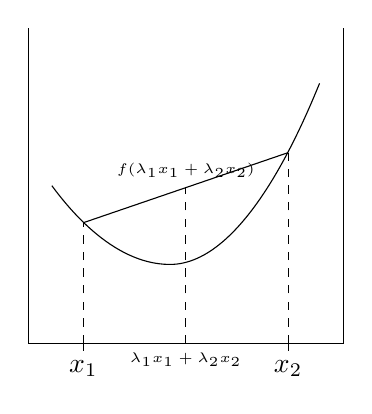
\begin{tikzpicture}
      \draw(-2, 4) -- (-2, 0) -- (2, 0) -- (2, 4);
      \draw (-1.3, 0.1) -- (-1.3, -0.1) node [below] {$x_1$};
      \draw (1.3, 0.1) -- (1.3, -0.1) node [below] {$x_2$};
      \draw (-1.7, 2) parabola bend (-.2, 1) (1.7, 3.3);
      \draw [dashed] (-1.3, 0) -- (-1.3, 1.53);
      \draw [dashed] (1.3, 0) -- (1.3, 2.42);
      \draw (-1.3, 1.53) -- (1.3, 2.42);
      \draw [dashed] (0, 0) node [below] {\tiny $\lambda_1x_1 + \lambda_2x_2$} -- (0, 1.975) node [above] {\tiny$f(\lambda_1x_1 + \lambda_2x_2)$};
    \end{tikzpicture}
  \end{center}
  A function is \emph{concave} if $-f$ is convex.
\end{defi}

\begin{prop}
  $f$ is convex if it is differentiable and $f''(x) \geq 0$ fora ll $x\in (a, b)$. It is strictly convex if $f''(x) > 0$.
\end{prop}

\begin{thm}[Jensen's inequality]
  If $f:(a, b) \to \R$ is convex, then
  \[
    \sum_{i = 1}^n p_i f(x_i) \geq f\left(\sum_{i = 1}^n p_ix_i\right)
  \]
  for all $p_1, p_2, \cdots, p_n$ such that $p_i \geq 0$ and $\sum p_i = 1$, and $x_i \in (a, b)$.

  This says that $\E[f(x)] \geq f(\E[X])$ (where $P(X=x_i) = p_i$).
\end{thm}

\begin{proof}
  It is true for $n = 2$ by the definition of convexity. Then
  \begin{align*}
    f(p_1x_1 + \cdots + p_nx_n) &= f\left(p_1x_1 + (p_2 + \cdots + p_n)\frac{p_2x_2 + \cdots + l_nx_n}{p_2 + \cdots + p_n}\right)\\
    &\leq p_1f(x_1) + (p_2 + \cdots p_n)f\left(\frac{p_2x_2 + \cdots + p_n x_n}{p_2 + \cdots + p_n }\right).\\
    &\leq p_1f_(x_1) + (p_2 + \cdots + p_n)\left[\frac{p_2}{(\;)}f(x_2) + \cdots + \frac{p_n}{(\;)}f(x_n)\right]\\
    &= p_1f(x_1) + \cdots + p_n(x_n).
  \end{align*}
  where the $(\;)$ is $p_2 + \cdots + p_n$.
\end{proof}

\begin{cor}[AM-GM inequality]
  Given $x_1, \cdots, x_n$ positive reals, then
  \[
    \left(\prod x_i\right)^{1/n} \leq \frac{1}{n}\sum x_i.
  \]
\end{cor}

\begin{proof}
  Take $f(x) = -\log x$. This is positive since its second derivative is $x^{-2}$.

  Take $\P(x = x_i) = 1/n$. Then
  \[
    \E[f(x)] = \frac{1}{n}\sum -\log x_i = -\log \text{GM}
  \]
  and
  \[
    f(\E[X]) = -\log \frac{1}{n}\sum x_i = -\log\text{AM}
  \]
  Since $f(\E[x]) \leq \E[f(x)]$, AM $\geq$ GM. Since $-\log x$ is strictly convex, AM $=$ GM only if all $x_i$ are equal.
\end{proof}

\begin{thm}[Cauch-Schwarz inequality]
  For any two random variables $X, Y$,
  \[
    (\E[XY])^2 \leq \E[X^2]\E[Y^2].
  \]
\end{thm}

\begin{proof}
  Assume $\E[Y^2] > 0$. Else $Y = 0$. Let
  \[
    w = X - Y\cdot \frac{\E[XY]}{\E[Y^2]}.
  \]
  Then
  \begin{align*}
    \E[w^2] &= \E\left[X^2 - 2XY\frac{\E[XY]}{\E[Y^2]} + Y^2\frac{(\E[XY])^2}{(\E[Y^2])^2}\right]\\
    &= \E[X^2] - 2\frac{(\E[XY])^2}{\E[Y^2]} + \frac{(\E[XY])^2}{\E[Y^2]}\\
    &= \E[X^2] - \frac{(\E[XY])^2}{\E[Y^2]}
  \end{align*}
  Since $\E[w^2] \geq 0$, the Cauchy-Schwarz inequality follows.
\end{proof}
\subsection{Covariance and correlation}
\begin{defi}[Covariance]
  Given two random variables $X, Y$, the \emph{covariance} is
  \[
    \cov(X, Y) = \E[(X - \E[X])(Y - \E[Y])].
  \]
\end{defi}

\begin{prop}\leavevmode
  \begin{enumerate}
    \item $\cov(X, c) = 0$ for constant $c$.
    \item $\cov(X + c, y) = \cov (X, Y)$.
    \item $\cov (X, Y) = \cov (Y, X)$.
    \item $\cov (X, Y) = \E[XY] - \E[X]\E[Y]$.
    \item $\cov (X, X) = \var (X)$.
    \item $\var (X + Y) = \var (X) + \var (Y) + 2\cov (X, Y)$.
    \item If $X$, $Y$ are independent, $\cov(X, Y) = 0$.
  \end{enumerate}
\end{prop}
These are all trivial to prove and proof is omitted.

Note that $\cov(X, Y) = 0$ does not imply they are independent.
\begin{eg}
  Let $(X, Y) = (2, 0), (-1, -1)$ or $(-1, 1)$ with equal probabilities of $1/3$. These are not independent since $Y = 0\Rightarrow X = 2$.

  However, $\cov (X, Y) = \E[XY] - \E[X]\E[Y] = 0 - 0\cdot 0 = 0$.

  Also if we randomly pick a point on the unit circle, and let the coordinates be $(X, Y)$, then $\E[X] = \E[Y] = \E[XY] = 0$ by symmetry. So $\cov(X, Y) = 0$ but $X$ and $Y$ are clearly not independent (they have to satisfy $x^2 + y^2 = 1$).
\end{eg}

\begin{defi}[Correlation coefficient]
  The \emph{correlation coefficient} of $X$ and $Y$ is
  \[
    \corr(X, Y) = \frac{\cov (X, Y)}{\sqrt{\var (X)\var (Y)}}.
  \]
\end{defi}
\begin{cor}
  $|\corr(X, Y)| \leq 1$.
\end{cor}

\begin{proof}
  Apply Cauchy-Schwarz to $X - \E[X]$ and $Y - \E[Y]$.
\end{proof}

\subsection{Markov inequality}
\begin{thm}[Markov inequality]
  If $X$ is a random variable with $\E|X| < \infty$ and $ a> 0$, then
  \[
    \P(|X| > a) \leq \frac{\E|X|}{a}.
  \]
\end{thm}

\begin{proof}
  We have
  \[
    I[\{|X|\geq a\}] \leq \frac{|X|}{a}.
  \]
  Since if $|X| \geq a$, then LHS = 1 and RHS $>$ 1; If $|X| \leq a$, then LHS = 0 and RHS is non-zero.
  
  Take the expected value to obtain
  \[
    \P(|X| \geq a) \leq \frac{\E |X|}{a}.
  \]
\end{proof}

\subsection{Chebyslev inequality}
\begin{thm}[Chebyslev inequality]
  If a $X$ is a random variable with $\E[X^2] < \infty$ and $\varepsilon > 0$, then
  \[
    \P(|X| \geq \epsilon) \leq \frac{\E[X^2]}{\varepsilon^2}.
  \]
\end{thm}

\begin{proof}
  We have
  \[
    I[\{|X|\geq \varepsilon\}] \leq \frac{x^2}{\varepsilon^2}.
  \]
  Then take the expected value and the result follows.
\end{proof}
\note that these not do not make any assumption about distributions of $X$.

\note If $\mu = \E[X]$, then
\[
  \P(|X - \mu| \geq \varepsilon) \leq \frac{\E[(X - \mu)^2]}{\varepsilon^2} = \frac{\var X}{\varepsilon^2}
\]

\subsection{Weak law of large numbers}
\begin{thm}[Weak law of large numbers (WLLN)]
  Let $X_1, X_2, \cdots$ be iid random variables, with mean $\mu$ and $\var \sigma^2$.
  
  Let $S_n = \sum_{i = 1}^n X_i$.

  Then for all $\varepsilon > 0$,
  \[
    \P\left(\left|\frac{S_n}{n} - \mu\right| \geq \epsilon\right) \to 0
  \]
  as $n\to \infty$.

  We say, $\frac{S_n}{n}$ tends to $\mu$ (in probability), or
  \[
    \frac{S_n}{n}\to_p \mu.
  \]
\end{thm}

\begin{proof}
  By Chebyshev,
  \begin{align*}
    \P\left(\left|\frac{S_n}{n} - \mu\right| \geq \epsilon\right)&\leq \frac{\E\left(\frac{S_n}{n} - \mu\right)}{\varepsilon^2}\\
    &= \frac{1}{n^2}\frac{\E(S_n -n\mu)^2}{\varepsilon^2}\\
    &= \frac{1}{n^2\varepsilon^2}\var (S_n)\\
    &= \frac{n}{n^2\varepsilon^2}\var (X_1)\\
    &= \frac{\sigma^2}{n\varepsilon^2} \to 0
  \end{align*}
\end{proof}

Note that we cannot relax the ``independent'' condition. For example, if $X_1 = X_2 = X_3 = \cdots = $ 1 or 0, each with probability $1/2$. Then $S_n/n \not\to 1/2$ since it is either 1 or 0.

\begin{eg}
  Suppose we toss a coin with probability $p$ of heads. Then
  \[
    \frac{S_n}{n} = \frac{\text{number of heads}}{\text{number of tosses}}.
  \]
  Since $\E[X_i] = p$, then the weak law of large number tells us that
  \[
    \frac{S_n}{n} \to p.
  \]
\end{eg}

\begin{thm}[Strong law of large numbers]
  \[
    \P\left(\frac{S_n}{n}\to \mu\text{ as }n\to \infty\right) = 1.
  \]
  We say
  \[
    \frac{S_n}{n}\to_{\mathrm{as}} \mu,
  \]
  where ``as'' means ``almost surely''.
\end{thm}
Proof is left for Part II because it is too hard.

\section{Probability generating functions.}
Consider a random variable $X$, taking values $0, 1, 2, \cdots$. Let $p_r = P(X = r)$.
\begin{defi}[Probability generating function (pgf)]
  The \emph{probability generating function (pgf)} of $X$ is
  \[
    p(z) = \E[z^X] = \sum_{r = 0}^\infty \P(X = r)z^r = p_0 + p_1z + p_2z^2\cdots = \sum_0^\infty p_rz^r.
  \]
  This is a power series (or polynomial), and converges if $|z| \leq 1$, since
  \[
    |p(z)| \leq \sum_r p_r |z^r| \leq \sum_r p_r = 1.
  \]
  We sometimes write as $P_X(z)$ to indicate the random variable.
\end{defi}

\begin{eg}
  Consider a fair die. Then $p_r = 1/6$ for $r = 1, \cdots, 6$. Then
  \[
    p(z) = \E[z^X] = \frac{1}{6}(z + z^2 + .., + z^6) = \frac{1}{6}z\left(\frac{1 - z^6}{1 - z}\right).
  \]
\end{eg}

\begin{thm}
  The distribution of $X$ is uniquely determined by its probability generating function.
\end{thm}

\begin{proof}
  $p_0 = p(0)$, $p_1 = p'(0)$ etc. (where $p'$ is the derivative of $p$) In general,
  \[
    \left. \frac{\d ^i}{\d z^i}p(z) \right|_{z = 0} = \frac{r!}{(r - i)!}p_i.
  \]
  So we can recover $(p_0, p_1, \cdots)$ from $p(z)$.
\end{proof}

\begin{thm}[Abel's lemma]
  \[
    \E[X] = \lim_{z\to 1}p'(z).
  \]
  If $p'(z)$ is continuous, then simply $\E[X] = p'(1)$.
\end{thm}

\begin{proof}
  \[
    p'(z) = \sum_1^\infty rp_r z^{r - 1} \leq \sum_1^\infty rp_r = \E[X].
  \]
  for $z \geq 1$. So
  \[
    \lim_{z\to 1}p'(z) \leq \E[X].
  \]
  If we pick $N$ large, then
  \[
    \sum_{1}^N rp_r \geq \E[X] - \varepsilon.
  \]
  So
  \[
    \E[X] - \varepsilon \leq \sum_1^N rp_r = \lim_{z\to 1}\sum _1^N rp_r z^r\leq \lim_{z \to 1} \sum_1^\infty rp_r z^r = \lim_{z\to 1} p' (z).
  \]
  So $\E[X] \leq \lim\limits_{z \to 1}p'(z)$.
\end{proof}

\begin{thm}
  \[
    \E[X(X - 1)] = \lim_{z \to 1}p''(z).
  \]
\end{thm}
\begin{proof}
  Same as above.
\end{proof}

\begin{eg}
  Consider the Poisson distribution. Then
  \[
    p_r = \P(X = r) = \frac{1}{r!}\lambda^r e^{-\lambda}.
  \]
  Then
  \[
    p(z) = \E[z^X] = \sum_0^\infty z^r \frac{1}{r!}\lambda^r e^{-\lambda} = e^{\lambda z}e^{-\lambda} = e^{\lambda(z - 1)}.
  \]
  We can have a sanity check: $p(1) = 1$, which makes sense, since $p(1)$ is the sum of probabilities.

  We have
  \[
    \E[X]= \left.\frac{\d }{\d z}e^{\lambda(z - 1)}\right|_{z = 1} = \lambda,
  \]
  and
  \[
    \E[X(X - 1)] = \left.\frac{\d ^2}{\d x^2}e^{\lambda(z - 1)}\right|_{z = 1} = \lambda^2
  \]
  So
  \[
    \var(X) = \E[X^2] - \E[X]^2 = \lambda^2 + \lambda - \lambda^2 = \lambda.
  \]
\end{eg}

\begin{thm}
  Suppose $X_1, X_2, \cdots, X_n$ are independent random variables with pgfs $p_1, p_2, \cdots, p_n$. Then the pgf of $X_1 + X_2 + \cdots + X_n$ is $p_1(z)p_2(z)\cdots p_n(z)$.
\end{thm}

\begin{proof}
  \[
    \E[z^{X_1 + \cdots + X_n}] = \E[z^{X_1}\cdots z^{X_n}] = \E[z^{X_1}]\cdots\E[z^{X_n}] = p_1(z)\cdots p_n(z).
  \]
\end{proof}

\begin{eg}
  Let $X\sim B(n, p)$. Then
  \[
    p(z) = \sum_{r = 0}^{n} \P(X = r)z^r = \sum \binom{n}{r} p^r(1 - p)^{n - r}z^r = (pz + (1 - p))^n = (pz + q)^n.
  \]
  So $p(z)$ is the product of $n$ copies of $pz + q$. But that is the pgf of $Y\sim B(1, p)$.

  This shows that $X = Y_1 + Y_2 + \cdots + Y_n$ (which we already knew).
\end{eg}

\begin{eg}
  If $X$ and $Y$ are independent Poisson random variables with parameters $\lambda, \mu$ respectively, then
  \[
    \E[t^{X + Y}] = \E[t^X]\E[t^Y] = e^{\lambda(t - 1)}e^{\mu(t - 1)} = e^{(\lambda + \mu)(t - 1)}
  \]
  So $X + Y\sim P(\lambda + \mu)$.

  We can also do it directly:
  \[
    P(X + Y = r) = \sum_{i = 0}^r \P(X = i, Y = r - i) = \sum_{i = 0}^r \P(X = i)\P(X = r - i),
  \]
  but is much more complicated.
\end{eg}

We can use pgf-like functions to obtain some combinatorial results.
\begin{eg}
  Suppose we want to tile a $2\times n$ bathroom by $2\times 1$ tiles. One way to do it is
  \begin{center}
    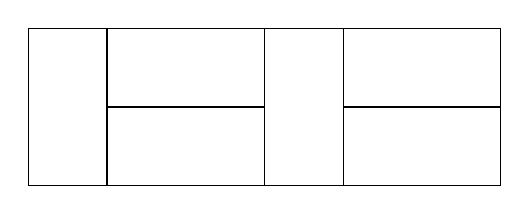
\begin{tikzpicture}
     \draw (0, 0) rectangle (6, 2);
     \draw (1, 0) rectangle (3, 1);
     \draw (1, 1) rectangle (3, 2);
     \draw (4, 0) rectangle (6, 1);
     \draw (4, 1) rectangle (6, 2);
    \end{tikzpicture}
  \end{center}
  We can do it recursively: suppose there are $f_n$ ways to tile a $2\times n$ grid. Then if we start tiling, the first tile is either vertical, in which we have $f_{n - 1}$ ways to tile the remaining ones; or the first tile is horizontal, in which we have $f_{n - 2}$ ways to tile the remaining. So
  \[
    f_n = f_{n - 1} + f_{n - 2},
  \]
  which is simply the Fibonacci sequence, with $f_0 = f_1 = 1$. 

  Let
  \[
    F(z) = \sum_{n = 0}^\infty f_nz^n.
  \]
  Then from our recurrence relation, we obtain
  \[
    f_nz^n = f_{n - 1}z^n + f_{n - 2}z^n.
  \]
  So
  \[
    \sum_{n = 2}^\infty f_n z^n = \sum_{n = 2}^{\infty} f_{n - 1}z^n + \sum_{n = 2}^\infty f_{n - 2}z^n.
  \]
  Since $f_0 = f_1 = 1$, we have
  \[
    F(z) - f_0 - zf_1 = z(F(z) - f_0) + z^2F(z).
  \]
  Thus $F(z) = (1 - z - z^2)^{-1}$. If we write
  \[
    \alpha_1 = \frac{1}{2}(1 + \sqrt{5}),\quad \alpha_2 = \frac{1}{2}(1 - \sqrt{5}).
  \]
  then we have
  \begin{align*}
    F(z) &= (1 - z - z^2)^{-1}\\
    &= \frac{1}{(1 - \alpha_1 z)(1 - \alpha_2 z)}\\
    &= \frac{1}{\alpha_1 - \alpha_2}\left(\frac{\alpha_1}{1 - \alpha_1 z} - \frac{\alpha_2}{1 - \alpha_2 z}\right)\\
    &= \frac{1}{\alpha_1 - \alpha_2}\left(\alpha_1 \sum_{n = 0}^\infty \alpha_1^nz^n - \alpha_2\sum_{n = 0}^\infty \alpha_2^n z^n\right).
  \end{align*}
\end{eg}

We can also consider \emph{Dyck words}, such as (), or  ((())()), ie any list of brackets that match (cf Lisp).

There is only one Dyck word of length 2, (). There are 2 of length 4, (()) and ()(). Similarly, there are 5 Dyck words of length 5.

Let $C_n$ be the number of Dyck words of length $2n$. Each Dyck word can be split written as $(w_1)w_2$, where $w_1$ and $w_2$ are Dyck words. Since the lengths of $w_1$ and $w_2$ must sum up to $2(n -1)$,
\[
  C_{n + 1} = \sum_{i = 0}^n C_iC_{n - i}.\tag{*}
\]
We again use pgf-like functions: let
\[
  c(x) = \sum_{n = 0}^\infty C_n x^n.
\]
From $(*)$, we can show that
\[
  c(x) = 1 + xc(x)^2.
\]
We can solve to show that
\[
  c(x) = \frac{1 - \sqrt{1 - 4x}}{2x} = \sum_0^\infty \binom{2n}{n}\frac{x^n}{n + 1},
\]
noting that $C_0 = 1$. Then
\[
  C_n = \frac{1}{n + 1}\binom{2n}{n}.
\]

\section{Conditional expectation}
\subsection{Conditional distribution and expectation}
\begin{defi}[Conditional distribution]
  Let $X$ and $Y$ be random variables (in general not independent) with joint distribution $P(X = x, Y = y)$. Then the \emph{marginal distribution} (or simply \emph{distribution} of $X$ is
  \[
    P(X = x) = \sum_{y\in \Omega_u}\P(X = x, Y = y).
  \]
  The \emph{conditional distribution} of $X$ given $Y$ is
  \[
    \P(X = x|Y = y) = \frac{\P(X = x, Y = y)}{\P(Y = y)}.
  \]
  The \emph{conditional expectation} of $X$ given $Y$ is
  \[
    \E[X|Y = y] = \sum_{x\int \Omega_X}x\P(X = x|Y = y).
  \]
  We can view this as a random variable: given a value of $Y$, we return the expectation of $X$.
\end{defi}

\begin{eg}
  Consider a dice roll. Let $Y = 1$ denote an even roll and $Y + 0$ denote an odd roll. Let $X$ be the outcome. Then $\E[X|Y] = 3 + Y$, ie 4 if even, 3 if odd.
\end{eg}

\begin{eg}
  Let $X_1, \cdots, X_n$ be iid $B(1, p)$. Let $Y = X_1 + \cdots + X_n$. Then
  \begin{align*}
    \P(X_1 = 1|Y = r) &= \frac{\P(X_1 = 1, \sum_{2}^n X_i = r - 1)}{\P(Y = r}\\
    &= \frac{p\binom{n - 1}{r - 1}p^{r - 1}(1 - p)^{(n - 1) - (r - 1)}}{\binom{n}{r} p^r (1 - p)^{n - 1}} = \frac{r}{n}.
  \end{align*}
  So
  \[
    \E[X_1|Y] = 1 \cdot \frac{r}{n} + 0\left(1 - \frac{r}{n}\right) = \frac{r}{n} = \frac{Y}{n},
  \]
  Showing that $\E[X|Y]$ is a random variable.
\end{eg}
\subsection{Properties of conditional expectation}
\begin{thm}
  If $X$ and $Y$ are independent, then
  \[
    \E[X|Y] = \E[X]
  \]
\end{thm}

\begin{proof}
  \begin{align*}
    \E[X|Y = y] &= \sum_{x}x\P(X = x|Y = y)\\
    &= \sum_x x\P(X = x)\\
    &= \E[X]
  \end{align*}
\end{proof}

We know that the expected value of a dice roll given it is even is 4, and the expected value given it is odd is 3. Since it is equally likely to be even or odd, the expected value of the dice roll is 3.5. This is formally captured by
\begin{thm}[Tower property of conditional expectation]
  \[
    \E_Y[\E_X[X|Y]] = \E_X[X],
  \]
  where the subscripts indicate what variable the expectation is taken over.
\end{thm}

\begin{proof}
  \begin{align*}
    \E_Y[\E_X[X|Y]] &= \sum_y \P(Y = y)\E[X|Y = y]\\
    &= \sum _y P(Y = y) \sum_{x}x\P(X = x|Y = y)\\
    &= \sum_x\sum_y x\P(X = x, Y = y)\\
    &= \sum _x x\sum_y \P(X = x, Y = y)\\
    &= \sum_x x\P(X = x)\\
    &= \E[X].
  \end{align*}
\end{proof}
This is also called the law of total expectation. We can state it as: suppose $A_1, A_2, \cdots, A_n$ is a partition of $\Omega$. Then
\[
  \E[X] = \sum_{i: \P(A_i) > 0}\E[X|A_i]\P(A_i).
\]
\subsection{Sums with a random number of terms}
We would like to consider a sum with a random number of terms. For example, an insurance company may receive a random number of claims, each demanding a random amount of money. Then we have a sum of a random number of terms.

\begin{eg}
Let $X_1, X_2, \cdots, X_n$ be iid with pgf $p(z) = \E{z^X}$. Let $N$ be a random variable independent of $X_i$ with pgf $h(z)$. What is the pgf of $S_n = X_1 + \cdots + X_N$?

\begin{align*}
  \E[z^{S_n}] &= \E[z^{X_1 + \cdots + X_N}]\\
  &= \E_N[\underbrace{\E_{X_i}<++>[z^{X_1 + \ldots + X_N}|N]}_{\text{assuming fixed }N}]\\
  &= \sum_{n = 0}^\infty \P(N = n) \E[z^{X_1 + X_2 + \cdots + X_n}]\\
  &= \sum_{n = 0}^\infty \P(N = n) \E[z^{X_1}] \E[z^{X_2}]\cdots\E[z^{X_n}]\\
  &= \sum_{n = 0}^\infty \P(N = n) (\E[z^{X_1}])^n\\
  &= \sum_{n = 0}^\infty \P(N = n) p(z)^n \\
  &= h(p(z))
\end{align*}
since $h(x) = \sum_{n = 0}^\infty \P(N = n) x^n$.

So
\begin{align*}
  \E[S_N] &= \left.\frac{\d }{\d z}h(p(z))\right|_{z = 1}\\
  &= h'(p(1))p'(1)\\
  &= \E[N]\E[X_1]
\end{align*}
To calculate the variance, use the fact that
\[
  \E[S_n(S_n - 1)] = \left.\frac{\d ^2}{\d z^2}h(p(z))\right|_{z = 1}.
\]
Then we can find that
\[
  \var (S_N) = \E[N]\var(X_1) + \E[X_1^2]\var(N).
\]
\end{eg}
\end{document} 
